\documentclass[journal, compsoc, 10pt]{IEEEtran}

\usepackage{graphicx}   								% \includegraphics[scale=]{}
\usepackage{subfigure}									% \subfigure[]{}
\usepackage{amsmath}									% \begin{split}			
\usepackage{amsthm}										% \begin{proof}
\usepackage{enumerate} 									% \begin{enumerate}
\usepackage[para,online,flushleft]{threeparttable} 		% \begin{threeparttable}
\usepackage{multirow}									% \multirow

\usepackage{algorithm}
%\usepackage{algorithmic}
\usepackage{algpseudocode}
\usepackage{amsmath}
\usepackage{amsfonts}
\usepackage{gensymb}
\usepackage{graphics}
\usepackage{epsfig}
\usepackage{ragged2e}
\usepackage{url}
\usepackage{color}
\usepackage[OT1]{fontenc}
\usepackage{caption}

\newtheorem{theorem}{Theorem}
\newtheorem{lemma}{Lemma}

\begin{document}

\title{DEAL: Distributed Energy-Aware Load Balancing Routing Algorithm for LEO Satellite Network}
\author{Chi-Yuan Huang and Guey-Yun Chang}

\IEEEcompsoctitleabstractindextext{%
\justify
\begin{abstract}
With the rise of network traffic demand, low-latency LEO satellite networks have become more popular.  The period of the satellite orbit can be divided into two: the sunlight period and the eclipse period. In the eclipse period, the satellite is only powered by its battery. Overusing a battery will lead to a high depth of discharge(DoD), which will lead to a shorter lifetime of the battery.  In Distributed Energy-Aware Load Balancing Routing Algorithm for LEO Satellite Network(DEAL), we proposed a method to estimate the remaining energy level of the neighbor satellite with little information demanded. Furthermore, DEAL also considers load balance.  DEAL can choose two shortest-path neighbors as the next hop, splitting the traffic flow into two by the status of the neighbor, and the status includes remaining energy, congestion level, and instability of ISL. We evaluated our algorithms by simulations on LEO satellite network with real Internet usage traces. The results showed DEAL can prolong the lifetime of the satellite battery, achieve a small occupying ratio of buffer queue, and a small link utilization ratio.

\end{abstract}

\begin{IEEEkeywords}
Satellites, Routing, Low earth orbit satellites, Orbits, Batteries.
\end{IEEEkeywords}}

\maketitle

%*******************************************************************************************************************
%*      Section 1                                                                                                     
%*******************************************************************************************************************
%%%%%%%%%%%%%%Introduction%%%%%%%%%%%%%%
\section{Introduction}
\label{ch:Introduction}
Satellite networks can provide coverage in all places on the earth, even the oceans, and deserts. Without terrain restrictions, communication between two cities becomes much more accessible through satellite technology. Thus people are getting more and more interest in satellite networks than terrestrial networks in a decade. According to different heights of orbit, we can divide satellites into three types: geostationary-earth orbit (GEO) satellite, medium earth orbit (MEO) satellite systems, and low-earth orbit (LEO) satellite. Compared to GEO satellite systems and MEO satellite systems, LEO satellite systems have higher throughput, higher data rate, and a lower orbit altitude, providing lower propagation delay and more possibility to achieve real-time communications\cite{AGENTBASED}. Therefore, researching LEO networks becomes popular in the field of satellite recently.

\subsection{Limits of LEO satellite}
Communication devices in satellites are typically powered by solar panels and battery cells, which are carefully designed to guarantee power supply and avoid deficiency\cite{CISCO}. When a LEO satellite spins around the earth, it will be covered periodically by the earth's shadow. Thus we can divide the LEO satellite orbital period into the solar period and eclipse period. When the sunlight can irradiate the satellite, it means the satellite is in the solar period. Otherwise, when the satellite is in the earth’s shadow, it means the satellite is in the eclipse period. When a satellite is in the eclipse period, the satellite’s energy consumption is relatively large. The battery is the only power supplier when a satellite is in the eclipse period. In contrast, the satellite is able to utilize solar energy directly in the solar period.

A battery's lifetime is affected by the depth of discharge(DoD). In many types of batteries, the total energy stored in the battery cannot be fully discharged without causing severe and often irreparable damage to the battery. Numerous cycles of use and more charge demanded on each cycle would lead to a shorter battery's lifetime. Moreover, the charge and discharge frequency of the LEO satellite is much higher than the frequency of the GEO satellite per day. The LEO satellite has an orbital period of 100 minutes. The eclipse period is 30–40 minutes per orbit, and it means that the LEO satellites can only use the battery's energy without charging for 30 to 40 minutes per cycle\cite{DOOR}. It may lead to an exceedingly low percentage of the battery's capacity. As far as the network lifetime is concerned, considering the DoD of the LEO satellite is necessary.

For instance, when we discharge the battery from 100\% to 20\% and then recharge back to 100\% which DoD is 80\%, the battery life cycle will be smaller than the battery discharged from 100\% to 70\%, and then recharge back to 100\% which DoD is 30\% \cite{TOWARDS}

Managing the power of a satellite is quite essential in a satellite network. If a battery runs out of cycles, the satellite will no longer work. Not only constructing and launching a satellite is very expensive, but exchanging batteries on satellites is also difficult \cite{LAUNCH}. People want to extend the life of a satellite to provide the service and lower the cost as much as possible.

\subsection{Benefits of saving satellite's energy}
Attaching importance to LEO's energy management is significant because it could be translated to cost-saving. The satellite, which needs lower energy, requires a smaller battery, smaller solar panels. Lighter hardware on the satellite would bring about saving costs on launching, and it will provide economic benefits. However, existing energy-efficient routing approaches on the Internet cannot be applied straightforwardly in satellite networks. It is necessary to understand these issues comprehensively and understand how network routings affect the lifetime of satellite networks. 

\subsection{Routing on satellite network}
Different from the terrestrial networks, the topology of constellation networks is usually sparse and deployed regularly.  and every satellite in this kind of network will cover plenty of users. Considering the un-uniform user distribution on earth surface, satellites in different orbit positions will encounter distinct density level. As a result, the traffic density will be distributed unbalanced in the satellite network.

A routing algorithm is a set of step-by-step operations used to direct Internet traffic efficiently. When the data leaves its source, many different paths it can take to its destination. Depending on whether the decision changes or not with time, the algorithm can be static or dynamic. In a satellite network, only dynamic solutions are meaningful because the high-speed movement of LEO satellites results in a dynamic change in satellite network topology.

A tranditional way to route on the LEO satellite network is to compute all the paths on the ground station centrally and then broadcast the information to all the satellites in the constellation. The satellites forward the data based on the routing table originally from the ground station. This centralized approach would be possible to find the optimal solution. However, this solution with a limited number of ground stations is challenging. The routing tables must be updated and sent to the satellites frequently. These updates require the ground-satellite link (GSL), but its intermittent availability can be insufficient to track the topology changes.

In addition, the total bandwidth has to be shared with other data. If the ground station frequently sends the routing information to the satellite to keep up with the topology change, it will occupy a specific bandwidth of GSL and ISL in the long term. Therefore, computing routes on the satellite itself is an approach to avoiding occupying the bandwidth of GSL

In addition, the total bandwidth has to be shared with other data. If the ground station frequently sends the routing information to the satellite to keep up with the topology change, it will occupy a specific bandwidth of GSL and ISL in the long term. Therefore, computing routes on the satellite itself is an approach to avoiding occupying the bandwidth of GSL.

Distributed routing refers to that every node on the network has the ability to decide the route of themselves and also requires the information of decision from each other. A simpler way for LEO constellation is a hop-by-hop autonomous routing. Each satellite could choose the next hop from the list of available links to route the packet in the best direction towards the destination. There is two motivation for this approach in the LEO network: first, increasing the resilience of the routing, with satellites able to run the routing algorithm independently of the rest of the network; on the other hand, exploiting the predictability of a LEO topology, where nodes do not move randomly, but according to well-known physical laws. The predictability allows skipping the "Hello" messages utilized to discover adjacent nodes in terrestrial ad-hoc networks. It minimizes the control information and overheads. Taking local decisions at each satellite also facilitates the management of congestion and failures in the network. A distributed algorithm can be run alone or used as a backup solution of more traditional routing table-based solutions.

A routing policy that uses only a single path is not necessarily optimal from the viewpoint of an entire network even though the path is the shortest one.
In order to balance the traffic load in the whole satellite network, most load balancing routing algorithm will collect link and traffic load states information and change/split the path for packets
and the traffic splitting mechanism plays an important role in traffic load balancing. Thus, in our scheme, every node in the network can split the traffic flow flexibly according to their neighbors' status such as traffic density, remaining energy, and the instability of ISLs to distribute the traffic, avoiding congestion.

%*******************************************************************************************************************
%*      Section 2                                                                                                     
%*******************************************************************************************************************
%%%%%%%%%%%%%%Related Work%%%%%%%%%%%%%%
\section{Related Work}

In this chapter, we will review previous the energy management and routing schemes for satellite network. 


\label{PRC}

\subsection{Energy Efficiency in Satellites}
\cite{BATTERYTYPE} proposed a design method such as, quantity and type, for solar panels and batteries to ensure that satellites that are launched and offline can perform all tasks without lack of power until the end of their life. In addition, under power management, they first classify the tasks to be performed by the satellites according to QoS. Then, without affecting the sufficiency of the power supply, they proposed a way to make the connected satellites perform the tasks as high as possible QoS version. First of all, in terms of design, they can reduce production costs and allocate more weight and space for effective payloads. In terms of management, they can maximize the task performance of a given power system design.

For another, more studies work on the management of missions to make use of energy more efficiently. Gatzianas et al. \cite{CROSSLAYER} proposed a cross-layer resource allocation scheme for wireless networks operating with rechargeable batteries, aiming to maximize total system utility.

Fu et al. \cite{ADMISSIONCONTROL} focused on the communication satellites with limited energy. They redesigned an energy allocation and admission control scheme to maximize the reward. 

\subsection{Routing in Satellite Networks}
\cite{INCOME} proposed using distributed routing scheme based on every ISL information like propagation delay, packet loss ratio, bandwidth and buffer length then use Shapley value to calculate the income distribution plan. Each satellite has its starting point to increase its maximum profit, that is, a satellite with a stronger processing capability to do the forwarding. \cite{LCD1} adopt hop-by-hop distributed routing schemes, and made rules for satellite to choose the next-hop without complex calculation. The main idea is basically trying to transmit in the same orbit to the same latitude of the destination satellite, performing cross-orbit transmission, and then making some changes according to the polar circle and seams in the rules. However, it does not consider the possible congestion of the inter-satellite link or the problem of satellite power because the satellite does not calculate other information. \cite{LCD2} and \cite{LCD3} are basically follow with same idea. However, still lots of study work on centralized routing scheme, because the movement of satellite is regular. \cite{CHARACTERISTICS} uses the movement characteristics of the satellite, the remaining time of each link can be calculated, combined with the path delay. If the link remaining time is less than the path delay, the routing table in the satellite node could be changed to the next handover satellite in advance, and the data packets sent on the link which is going to be changed will be stopped, thereby avoiding the packets lost caused by the switching in the link. \cite{LOWTRACK} calculated the propagation delay, packet loss ratio, and bandwidth between links, finding the candidate paths according to the upper limit of hops, and then use the GWO algorithm to find the best route. \cite{PRIORITY} proposed an operation center on the ground calculates the routes according to the priority, bandwidth, remaining time of links. And it creates not only just one route but backup routes to solve link failure or congestion. But these routing schemes, either centralized or distributed, didn’t consider the energy of the satellite. Even if we don't consider the lifetime of the constellation, it is possible when the data sent to a satellite that lacks energy.


\subsection{Energy-Efficient Routing in the LEO network}

\cite{LOCATIONAWARE} proposed a concept of the satellite's location with sun period and eclipse period, it first computes all the possible routes and all the propagation delay of inter-plane ISLs and intra-plane ISLs. Then it sums up all propagation delay of links whose transmitter satellites are in the eclipse period. The cost of a route is computed by two main delays: the sum of all propagation delays and the sum of propagation delays in the eclipse period. And there will be a weighting factor to determine which part the user pays more attention to. If the weighting factor of the first part is bigger, the route computation will focus on finding the route which propagation delay is small, otherwise, the route computation will focus on saving energy. Thus the algorithm can provide a trade-off between the operational lifetime of the satellite networks and the propagation delay of the selected routes. By sacrificing some propagation delay, this method can achieve a kind of load balance. 
\cite{TOWARDS} proposed an algorithm that computes link costs iteratively to compute a routing that minimizes the total recharge/discharge cycle number. It can also turn the satellite which is not needed temporarily into sleep mode, which means the satellite will shut down partial power for some components temporarily. \cite{QOS} thought that service should be classified to make the best use of the network utility, and the algorithm also brings the concept of energy to make sure any reliable data has been sent. Nevertheless, all these schemes are centralize routing, and if any link failure occurs, the route cannot be updated immediately.

%*******************************************************************************************************************
%*      Section 3                                                                                                     
%*******************************************************************************************************************
%%%%%%%%%%%%%%Preliminary%%%%%%%%%%%%%%
\section {System Model}
\label{sec:SYS}

\subsection{Network Topology}
We construct an satellite constellation in \ref{fig:TOPOLOGY}, a polar-orbiting LEO constellation consisting of $w$ low earth orbits and $h$ satellites per orbit. It can provide global coverage at 24 hours. The links between any two satellites call inter-satellite links (ISLs). Because the satellites move in opposite directions will lead to a severe doppler shift, we assume there are no cross-seam ISLs. Therefore, every satellite has four interfaces\cite{4ISL} to construct ISLs with other satellites except for the satellites along the counter-rotating seam; two are intra-plane ISLs, formed by the identical orbit and two adjacent satellites; the others are inter-plane ISLs, formed by two satellites in neighbor orbits. If a satellite moves into the polar region, its inter-plane ISL is disconnected temporarily due to the physical limits such as antenna tracking, while the intra-plane ISLs are maintained on all occasions.

\begin{figure}[H]
	\centering
	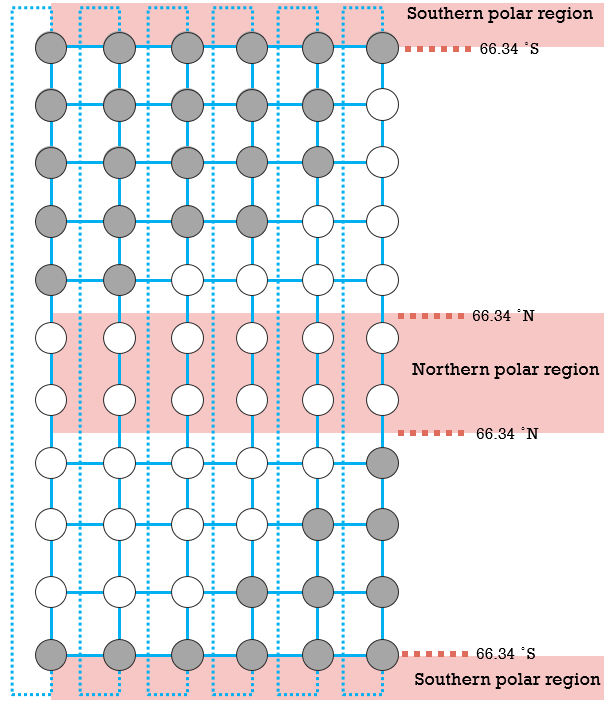
\includegraphics[scale=0.9,clip, width=0.5\textwidth]{fig/Topology.png}	
	\caption{Topology of satellite network}
	\label{fig:TOPOLOGY}
\end{figure}

The satellite network topology is regular because the movements of satellite follow the laws of motion. Then we discretize the continuously changing topology structure into several time intervals $\Delta t =[t_0, t_1], [t_1, t_2],...,[t_{n-1}, t_n]$. The labels will not change in each interval.

The LEO satellite position can be predicted/determined by Two Line Element (TLE). TLE is a data format encoding a list of orbital elements of an Earth-orbiting object for a given point in time and is made publicly by the Joint Space Operations Center(JSpOC). The local satellite can obtain the TLE of the satellites in the constellation from the ground periodically(about 6 hours \cite{TLE}).

The satellites on polar-orbit will occur counter-rotating, which means two satellites move in opposite directions. The mean orbital velocity of a LEO satellite is about 7.8 km/s.  Two satellites move at high speed and in the opposite directions will lead to a severe Doppler shift, called "seam." Communication with cross-seam ISLs is costly. In this paper, we view it as disconnected\cite{COUNTERROTATING}.

\subsection{Traffic Density Model}
The surface of the earth is divided into $j \times 2j$ grids  and calculated the population density of every grid\cite{TRAFFICDENSITY}, shown in \ref{fig:TRAFFICDENSITY}]. Then every grid $g_i$ obtains a density level $\rho_i$ of traffic.

\begin{figure}[H]
	\centering
	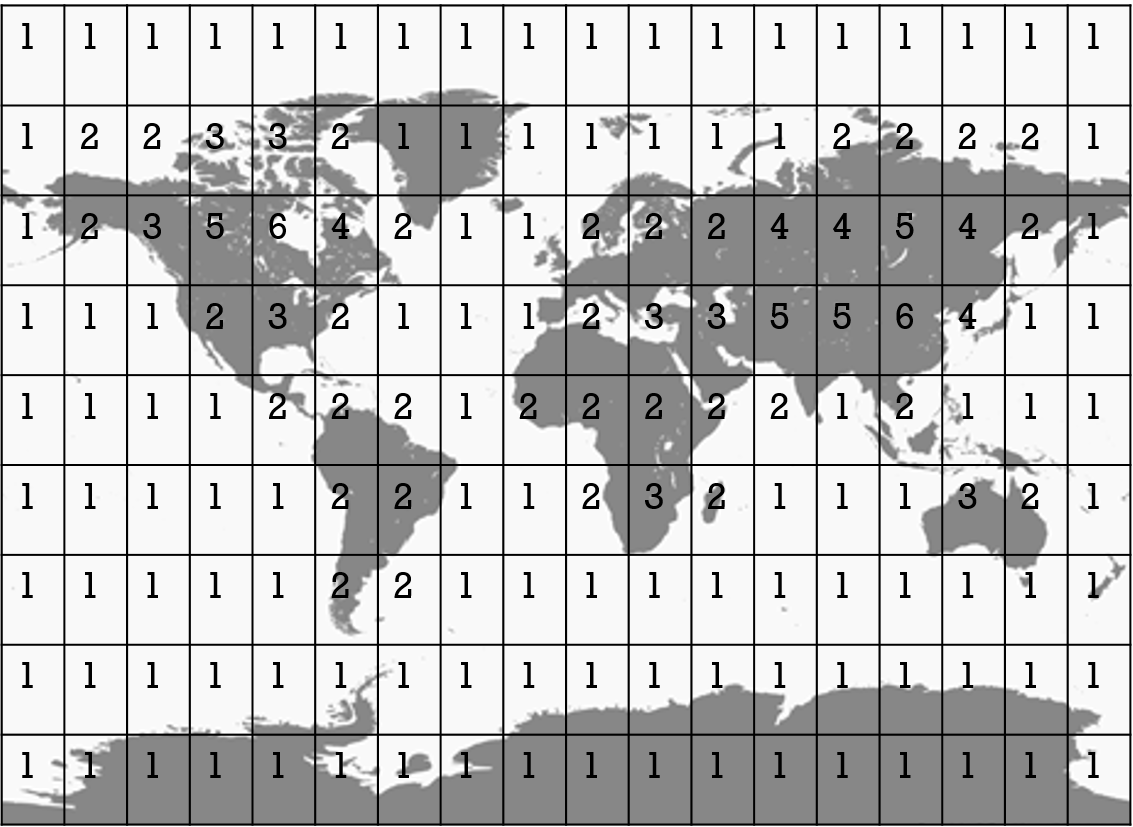
\includegraphics[scale=0.9,clip, width=0.5\textwidth]{fig/TrafficDensity.png}	
	\caption{Density level on grid map}
	\label{fig:TRAFFICDENSITY}
\end{figure}

The density level $\rho$ of each grid is calculated as:
\begin{equation}
 l_{a} \approx \frac{R \pi}{j} \cos \left(\theta_{\text {grid }}\right) 
\end{equation}

\begin{equation}
 l_{b} \approx \frac{R \pi}{j} 
\end{equation}

\begin{equation}
 A \approx l_{a} l_{b}=\left(\frac{R \pi}{j}\right)^{2} \cos \left(\theta_{g r i d}\right) 
\end{equation}

\begin{equation}
 \rho=\frac{N_{u}}{A} 
\end{equation}

where $A$ represents the area of each grid, $\theta_{grid}$ is the center latitude value of each grid, $R$ is the Earth radius, $l_{a}$ and $l_{b}$ corresponding to the length of each grid along the longitude and latitude direction, and $N_u$ is the number of users in the grid. Then each vertical projection of the satellite onto the surface of the Earth can be mapped to one of the grids, and it denoted each satellite has a traffic density level $D_n$.

%*******************************************************************************************************************
%*      Section 4                                                                                                     
%*******************************************************************************************************************
%%%%%%%%%%%%%%Methodology%%%%%%%%%%%%%%
\section{Methodology}


\subsection{Overview}
\label{sec:LEOMDL}

Satellites are assumed to be geometry awareness, i.e., knowledge of the topology and geometry and dynamics of the network are available to satellites. Satellites, even in small satellites with limited processing capacity, are geometry awareness because Attitude and Determination and Control subsystem (ADCS), which is used to point to neighbor satellites for intersatellite communication, shall rely on geometry awareness.

We adopt hop-by-hop shortest path routing based on Manhattan distance. Every node has two neighbors on the shortest path to the destination, except for the source node and the destination node are on the same orbit or same row, there may not exist two neighbors on the shortest path to the destination. In that case, we only choose the shortest one to avoid route oscillation.

Before a transmission, every node chooses one of the two neighbors according to the status that includes the remaining power, congestion level, and the instability of ISL.

The cost when a local satellite chooses a neighbor satellite $S_n$ as its next hop can be calculated as below.

\begin{equation}
	Cost_{n}=C_{n}+k \cdot P_{n}+I_{n}
\end{equation}
where $C_n$ is the congestion level of satellite $S_n$, $P_n$ is the power burden of satellite $S_n$ and $I_n$ is the instability of $S_n$.
Weighting factor $k=1-\frac{MD(S_n,\ D)}{d}$ blongs to $[0,1]$,  where $MD(S_n,\ D)$ is the Manhattan distance between satellite $S_n$ and the destination satellite, and $d$ is the diameter of the network (which is a constant). The times of splitting flow increases with distance, so  $k$, which represents the significance of energy, should increase hop-by-hop. Then $Cost_1$ and $Cost_2$ are the costs of the two neighbors, $S_1$ and $S_2$ repectively. The probability of sending a packet to $S_1$ is $\frac{Cost_2}{Cost_1+Cost_2}$ and to $S_2$ is $\frac{Cost_1}{Cost_1+Cost_2}$.


\subsection{ISL Instability}
Owing to the physical limits of the antenna, the link stability between two  satellites depends on their relative distance and velocity \cite{ISL1}\cite{ISL2}.
Intra-plane ISLs are stable because the distance is nearly constant but inter-plane ISLs are unstable because the distance and the relative velocity change with latitude. Clearly, the distance of inter-plane ISL is: 

\begin{equation}
 \operatorname{dist}\left(l a t^{\circ}\right)=r \sqrt{2} \cos \left(l a t^{\circ}\right) \cdot \sqrt{1-\cos \left(360^{\circ} \frac{1}{2 w}\right)} 
 \label{eq:INTERISL}
\end{equation}

where $r$ is the radius of the plane, $lat^{\circ}$ stands for the latitude at which the center of the ISL resides, and $w$ is the number of orbits.

And we define the function of normalizing instability of inter-plane ISL is:
\begin{equation}
 I\left(l a t^{\circ}\right)=\frac{\operatorname{dist}\left(l a t^{\circ}\right)-\operatorname{dist}\left(66.34^{\circ}\right)}{\operatorname{dist}\left(0^{\circ}\right)-\operatorname{dist}\left(66.34^{\circ}\right)} \cdot M A X^{\lambda} 
 \label{eq:NORMALIZEDINSTABILITY}
\end{equation}

\begin{equation}
 \lambda=\left\{\begin{array}{ll}1, & \text { opposite direction / in polar region } \\ 0, & \text { same direction }\end{array}\right. 
\end{equation}

where $\lambda \in \{0,1\}$, if $\lambda = 1$ , it represents the two satellites move in the opposite directions or one of the satellites is in the polar region. if $\lambda = 0$, it means that two satellites move in the same direction and both of them are not in the polar region, and $MAX$ is an extremely large number.

Then the instability $I_n$ of local satellite ISL to satellite $S_n$ is defined as follows. 
\begin{equation}
 I_{n}=\left\{\begin{array}{ll}I\left(l a t_{n}^{\circ}\right), & \text { inter-plane ISL } \\ 0, & \text { intra-plane ISL }\end{array}\right. 
 \label{eq:INSTABILITY}
\end{equation}

Notice that the intra-plane ISL is stable, so $I_n$ always equals 0 on intra-plane ISL.

\subsection{Energy Burden of Satellite}
\subsubsection{Energy level of satellite}
Although neighboring satellites could acquire the status of each other by the "Hello message" \cite{OPSPF},  frequently exchanging hello message is still bandwidth consuming and  may make the congestion on links more severe. Hence, we make use of the satellite historical position information to estimate the remaining energy.

During eclipse time, when satellites pass through a shadow region on the opposite side of the earth from the sun, satellites are powered by batteries. The longer time a satellite in the eclipse area (the shadow of the Earth), the more power of satellite's battery is consumed. There are two common ways to acquire satellite energy information: First, every satellite will flood its energy status to the whole network periodically. Second, the satellite will tell the ground station or GEO satellites their energy status, then other satellites can obtain the energy status through the ground station or the GEO satellites. 

Although state of health (e.g, energy level information) of satellites are usually periodically transmitted to ground server or GEO, due to limit density of ground server and bandwidth consumption,  energy level information (e.g., state of charge) of other satellites are not available.  To prolong of satellite life time, energy level of neighboring statellites are also considered in our scheme. 

We use TLE of neighboring satellites to estimate their remaining energy level. 
In Figure \ref{fig:ELLIPSE}, the projection of the Earth’s shadow on the orbital plane of an satellite is an ellipse. Refer to \cite{ELLIPSE}, the semi-minor axis $b$ and semi-major axis $a$ of the ellipse are denoted as $b=R$ and $a=R\ csc\ i$, respectively, where $R$ is the radius of the earth and $i$ defines the inclination of the Sun onto the orbital plane of the satellite. The equation of an ellipse is given by 

\begin{equation}
 \delta^{2}=\frac{b^{2}}{1-e^{2}(\cos \theta)^{2}} 
 \label{eq:ELLIPSE}
\end{equation}
where $\delta$ is the distance from the center to either vertex of the ellipse, and $\theta = \angle SOC$, measured in the orbit plane between the satellite $S$ and the conjunction point $C$ (the intersection of the satellite orbit and the straight line between the Earth and Sun).

The eccentricity of an ellipse is given by
\begin{equation}
 e=\frac{\sqrt{a^{2}-b^{2}}}{a}
 \label{eq:ECCENTRICITY}
\end{equation}

\begin{figure}[H]
	\centering
	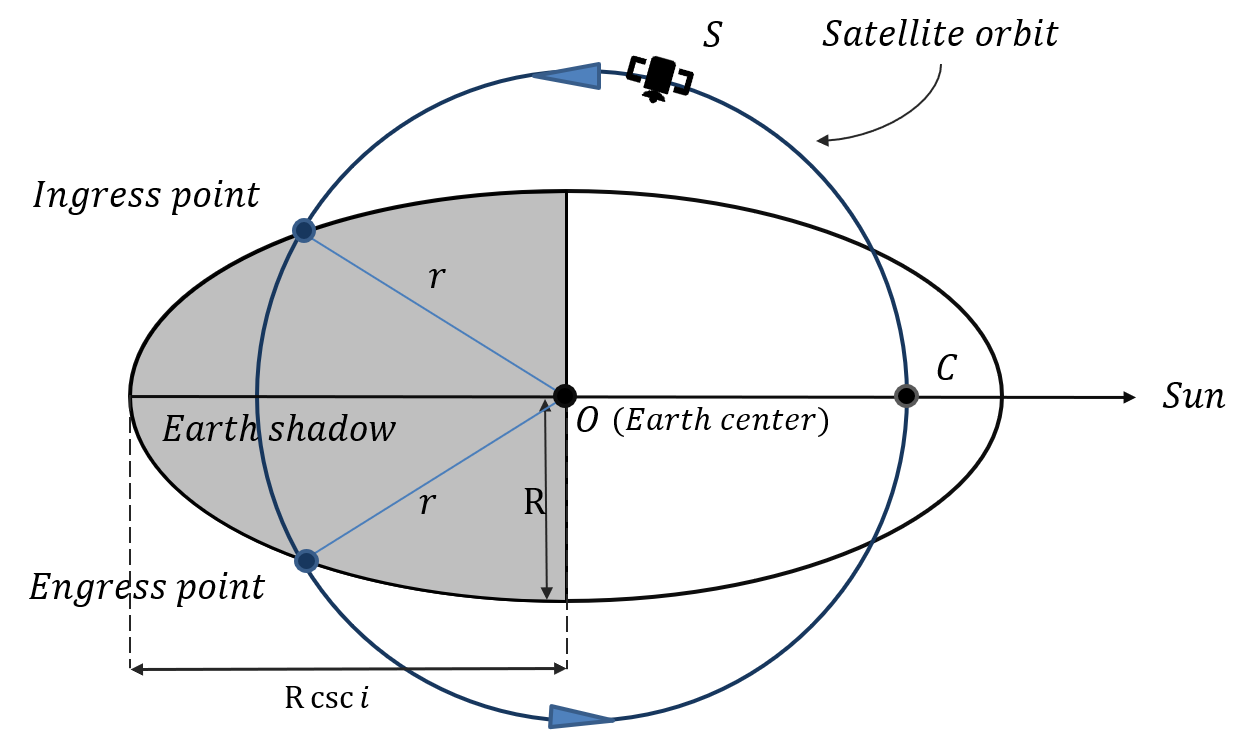
\includegraphics[scale=0.9,clip, width=0.4\textwidth]{fig/ellipse.png}	
	\caption{The shadow area, the angle of ingress/egress.}
	\label{fig:ELLIPSE}
\end{figure}

Substituting $a=R\ csc\ i$ and $b=R$ into eq(eccentricity). After little reduction, yields 

\begin{equation}
 e=\cos i 
\end{equation}

The ingress/egress point is when the distance between a point on the ellipse edge and the ellipse center equals the radius of the satellite orbit $r$.
Then the equation  \ref{eq:ELLIPSE} can be written as:
\begin{equation}
 \delta_{i n}^{2}=r^{2}=\frac{R^{2}}{1-(\cos i)^{2}\left(\cos \theta_{i n}\right)^{2}} 
\end{equation}

where $\delta^2_{in}$ is the distance between the ingress and the center of earth, and $\theta_{in}$ is the angle when the satellite enters the shadow. Clearly, we have

\begin{equation}
 \cos \theta_{i n}=\pm \sqrt{\frac{1-\left(\frac{R}{r^{2}}\right)^{2}}{\cos i}} 
\end{equation}

The duration angle of a circular orbit satellite in the eclipse is $\theta_E$, denoted as
\begin{equation}
 \theta_{E}=2\left(180^{\circ}-\theta_{i n}\right) 
 \label{eq:DURATONANGLE}
\end{equation}

Now the shadow interval can be obtained from
\begin{equation}
 t_{S H}=\frac{\theta_{E}}{360^{\circ}} \cdot P 
 \label{eq:SHADOWINTERVAL}
\end{equation}
where $P$ is the period of the satellite.

We set the $\theta = 0^{\circ}$ as the start of a period,**then the time of a satellite entering the eclipse is 
\begin{equation}
 t_{\text {enter }}=\frac{\theta_{\text {in }}}{360^{\circ}} P 
 \label{eq:ENTERINGTIME}
\end{equation}

Let $S_{n,t_{d}}^{\text {energy }}$ represent the total energy consumption of satellite $S_n$ in the $t_{d}$ time.
\begin{equation}
 T_{d}=t_{\text {current }}-t_{\text {enter }} 
\end{equation}

where $t_{current}$ is the current time.

In every time slot, satellite $S_n$ will obtain a traffic density level mapped to the ground. In this work, we viewed the traffic density level as the power consumption since the traffic density is significantly positively correlated with the power consumption. Thus the estimated power consumption of satellite $S_n$ can be the sum of the traffic density level in the $t_{d}$ time:
\begin{equation}
 S_{n, t_{d}}^{\text {energy }}=\sum_{t=t_{e n t e r}}^{t_{d}} D_{n}^{t} 
\label{eq:ENERGYCONSUMPTION}
\end{equation}

where $D_n^t$ is the density level of satellite $S_n$ at time $t$.
Then we normalized the power consumption to
\begin{equation}
  \frac{S_{n, t_{d}}^{\text {energy }}-\min S_{n,t_{d}}^{\text {energy }}}{maxS_{n,t_{d}}^{\text {energy }}-\min S_{n,t_{d}}^{\text {energy }}}
\label{eq:ENERGYCONSUMPTION}
\end{equation}

\subsubsection{Orbit Section}
Except for estimating the power consumption of satellites, we take a step further by classifying the energy burden of using a satellite in different sections of an orbit.
We divide an orbit into 4 sections:

\begin{itemize}
  \item Sunlight section
  \item Just entered the eclipse section
  \item Middle of the eclipse section
  \item About to leave the eclipse section
\end{itemize}

\paragraph{Sunlight section}
In the sunlight section, the satellite is powered by sunlight, and the battery is also being charged, so the remaining energy of battery is sufficient.

\paragraph{Just entered the eclipse section}
The satellite is powered by a battery but the satellite just entered the eclipse area, so the remaining battery power is regarded as sufficient as well.
\begin{equation}
  if\  \frac{t_{\theta_{n}}-t_{\text {enter }}}{t_{S H}}<\frac{1}{3} \rightarrow  just\ entered\ the\ eclipse\ section
\end{equation}

where $t\theta_n$ is the angle of satellite $n$ of current time,  $t_{\theta_n}-t_{enter}$ can be represented how long has a satellite been in the eclipse time.

\paragraph{Middle of the eclipse section}
The satellite is powered by a battery, and the satellite has already entered the eclipse area for a while; thus, the remaining battery power is relatively viewed as less.
\begin{equation}
  if\  \frac{t_{\theta n}-t_{\text {enter }}}{t_{S H}}<\frac{2}{3} \rightarrow  middle\ of\ the\ eclipse\ section
\end{equation}

\paragraph{About to leave the eclipse section}
The satellite is powered by a battery, and the satellite has already entered the eclipse area for a long time; thus, the remaining battery power is less than the satellite in the middle of the eclipse zone. In this paper, we focus on the DoD of the battery issue, so we should not view the satellite in this zone as a proper next hop.
\begin{equation}
  if\  \frac{t_{\theta_{n}}-t_{\text {enter }}}{t_{S H}}<1 \rightarrow  about\ to\ leave\ the\ eclipse\ section
\end{equation}

After we divide the area of the eclipse, the concept of remaining energy can be transformed into the burden of using per satellite.
Every section is assigned to a burden factor $\gamma$ between 0 and 1. The satellite's power burden is positively correlated with the burden factor. For example, when a satellite is in the sunlight section, which will not consume the battery power, its burden factor is 0. The expression and the burden factor of each section is shown in \ref{table:SECTION}.

\begin{table*}[h]
	\caption{Burden factor of section and the expression}
	\label{table:SECTION}
\begin{center}
\begin{tabular}{|l|l|l|}
\hline
\textbf{Section} & \textbf{Expression}      &  \textbf{Burden factor($\gamma$)}          \\  \hline
Sunlight section           			  & $ \cos \theta_{n}>\sqrt{\frac{1-\left(\frac{q}{q_{S H}}\right)^{2}}{\cos i}} $ or $ \cos \theta_{n}<-\sqrt{\frac{1-\left(\frac{q}{q_{S H}}\right)^{2}}{\cos i}} $  & 0.0  	\\ \hline
Just entered the eclipse section                   & $ \frac{t_{\theta n}-t_{\text {enter }}}{t_{S H}}<\frac{1}{3} $          													      &0.25	 \\ \hline
Middle of the eclipse section                      & $ \frac{1}{3}<\frac{t_{\theta n}-t_{e n t e r}}{t_{S H}}<\frac{2}{3} $               											      &0.5	\\ \hline
About to leave the eclipse section              & $ \frac{2}{3}<\frac{t_{\theta n}-t_{\text {enter }}}{t_{S H}}<1 $             												      &0.75	 \\ \hline

\end{tabular}
\end{center}
\end{table*}

Therefore, if we want to use satellite $S_n$ as the next hop, we not only have to consider its remaining energy but its current zone of eclipse. 
Here we define the potential energy risk as the probability of a satellite runs out of battery. We quntify the potential energy risk of Satellite $S_n$ is:
\begin{equation}
 P_{n}=\left(\frac{S_{n, t_{d}}^{\text {energy }}-\min S_{n, t_{d}}^{\text {energy }}}{\max S_{n, t_{d}}^{\text {energy }}-\min S_{n, t_{d}}^{\text {energ }}}\right) \cdot \gamma_{n},
\label{eq:POTENTIALENERGYRISK}
\end{equation}

where $\gamma_n$ is the burden factor of satellite $S_n$.
With the rise of the potential energy risk, a battery gets easier to become a high-DoD battery which will lead to a shorter life time.


\subsection{Congestion Level}
To estimate congestion level of satellites, we use the Discounting Rate Estimator (DRE) \cite{CONGA} , 
which is  similar to calculating an exponential moving average but is easier to implement,  and reacts faster to traffic bursts. 
In table[c], each satellite maintains a register, $V_n$ for each neighboring satellite $V_n$. 
$V_n$ is incremented for each packet sent to $V_n$  and is decremented periodically (every $T_{dre}$) with a multiplicative factor $\alpha$ between $0$ and $1$. More precisely,
\begin{equation}
 V_{n} \leftarrow V_{n} \times(1-\alpha) 
\label{eq:CONGA}
\end{equation}

So $V_n$ is proportional to the rate of traffic over the link to $S_n$. If the traffic rate is $Q_n$, then $V_n\approx Q_n \cdot \tau$, where $\tau = \frac{T_{dre}}{\alpha}$. The round trip time(RTT) of satellites is in 30ms to 50ms \cite{TELESAT}, and $T_{dre}$ could be a little larger than the RTT time.

Then the congestion level of neighboring satellite $S_n$ is calculated as:
\begin{equation}
 C_{n}=\frac{2 \cdot a \tan \left(V_{n} \cdot D_{n}\right)}{\pi} ,
\end{equation}

where $C_n$ is between $0$ and $1$, and $D_n$ is the density level of satellite $S_n$.





%*******************************************************************************************************************
%*      Section 5                                                                                                     
%*******************************************************************************************************************
%%%%%%%%%%%%%%Performance Analysis%%%%%%%%%%%%%%
%\input{Performance Analysis}

%*******************************************************************************************************************
%*      Section 6                                                                                                     
%*******************************************************************************************************************
%%%%%%%%%%%%%%Simulation%%%%%%%%%%%%%%
\section{Performance Evaluation}
We use Omnet++(5.6.2) as the primary network simulation platform and evaluate the performance of our method and SPF[2] in terms of packet delivery ratio, link utilization, times of dropping packets, occupying ratio of the queue, remaining battery, and end-to-end delay in the satellite network whose constellation type is Walker[3].

\subsection{Simulation Parameters}
The simulation parameters are shown in \ref{table:PARAMETERS}. Each satellite is assumed to have four ISLs with two intra-orbits ISLs and two inter-orbits ISLs. The packet size is fixed to 1000 bits. In each packet transmission, it will cost 0.7 joules on transmitter satellite and 0.4 joules on receiver satellite per packet. The number, the source, and the destination of packets will be generated randomly based on the population distribution \cite{TRAFFICDENSITY}.

\begin{table*}[h]
	\caption{Simulation Parameters}
	\label{table:PARAMETERS}
\begin{center}
\begin{tabular}{|l|l|}
\hline
\textbf{Parameters} & \textbf{Values}           \\  \hline
Constellation type            & Walker          \\ \hline
Orbital height                & 780 km          \\ \hline
Number of orbital planes      & 6               \\ \hline
Number of satellites in orbit & 11              \\ \hline
Orbital inclination           & 86.4°           \\ \hline
Packet size                   & 1000 bits       \\ \hline
Initial battery energy        & 5000 joules     \\ \hline
Transmission required energy  & 0.7  joules     \\ \hline
Reception required energy     & 0.4  joules     \\ \hline
$\alpha$                      & 0.5             \\ \hline
$T_{dre}$                     & 0.06 ms       \\ \hline
\end{tabular}
\end{center}
\end{table*}

\subsection{Impact of Queue Size}
We first evaluate the relationship between queue length of the receiver satellite and the packet delivery ratio. The channel data rate is 10Mbps, and the unit of the queue is one packet (i.e., 1000 bits). \ref{fig:QUEDELIVERY} shows the delivery ratio for the examined schemes and various queue length. We can see both delivery ratios of the two schemes rise with the increased length of the queue since the packet has a longer time to keep in the queue and be processed. However, the growth rate of DEAL is higher than SPF's. This is because in DEAL, we split the traffic flow to avoid congestion, i.e., avoid sending all packets with the same link/path.  The modeling results suggest that DEAL achieves lower queue lengths than SPF.

To observe the probability of congestion and the pressure of queue, we evaluate the mean occupying ratio of two schemes. \ref{fig:QUEOCCUPYING} shows the mean occupying ratio of the queue with various queue length. Clearly, the higher the occupying ratio of a queue is, the higher the probability of dropping a packet is. 

\begin{figure}[htp]
	\centering
	\subfigure[]{
		\centering
		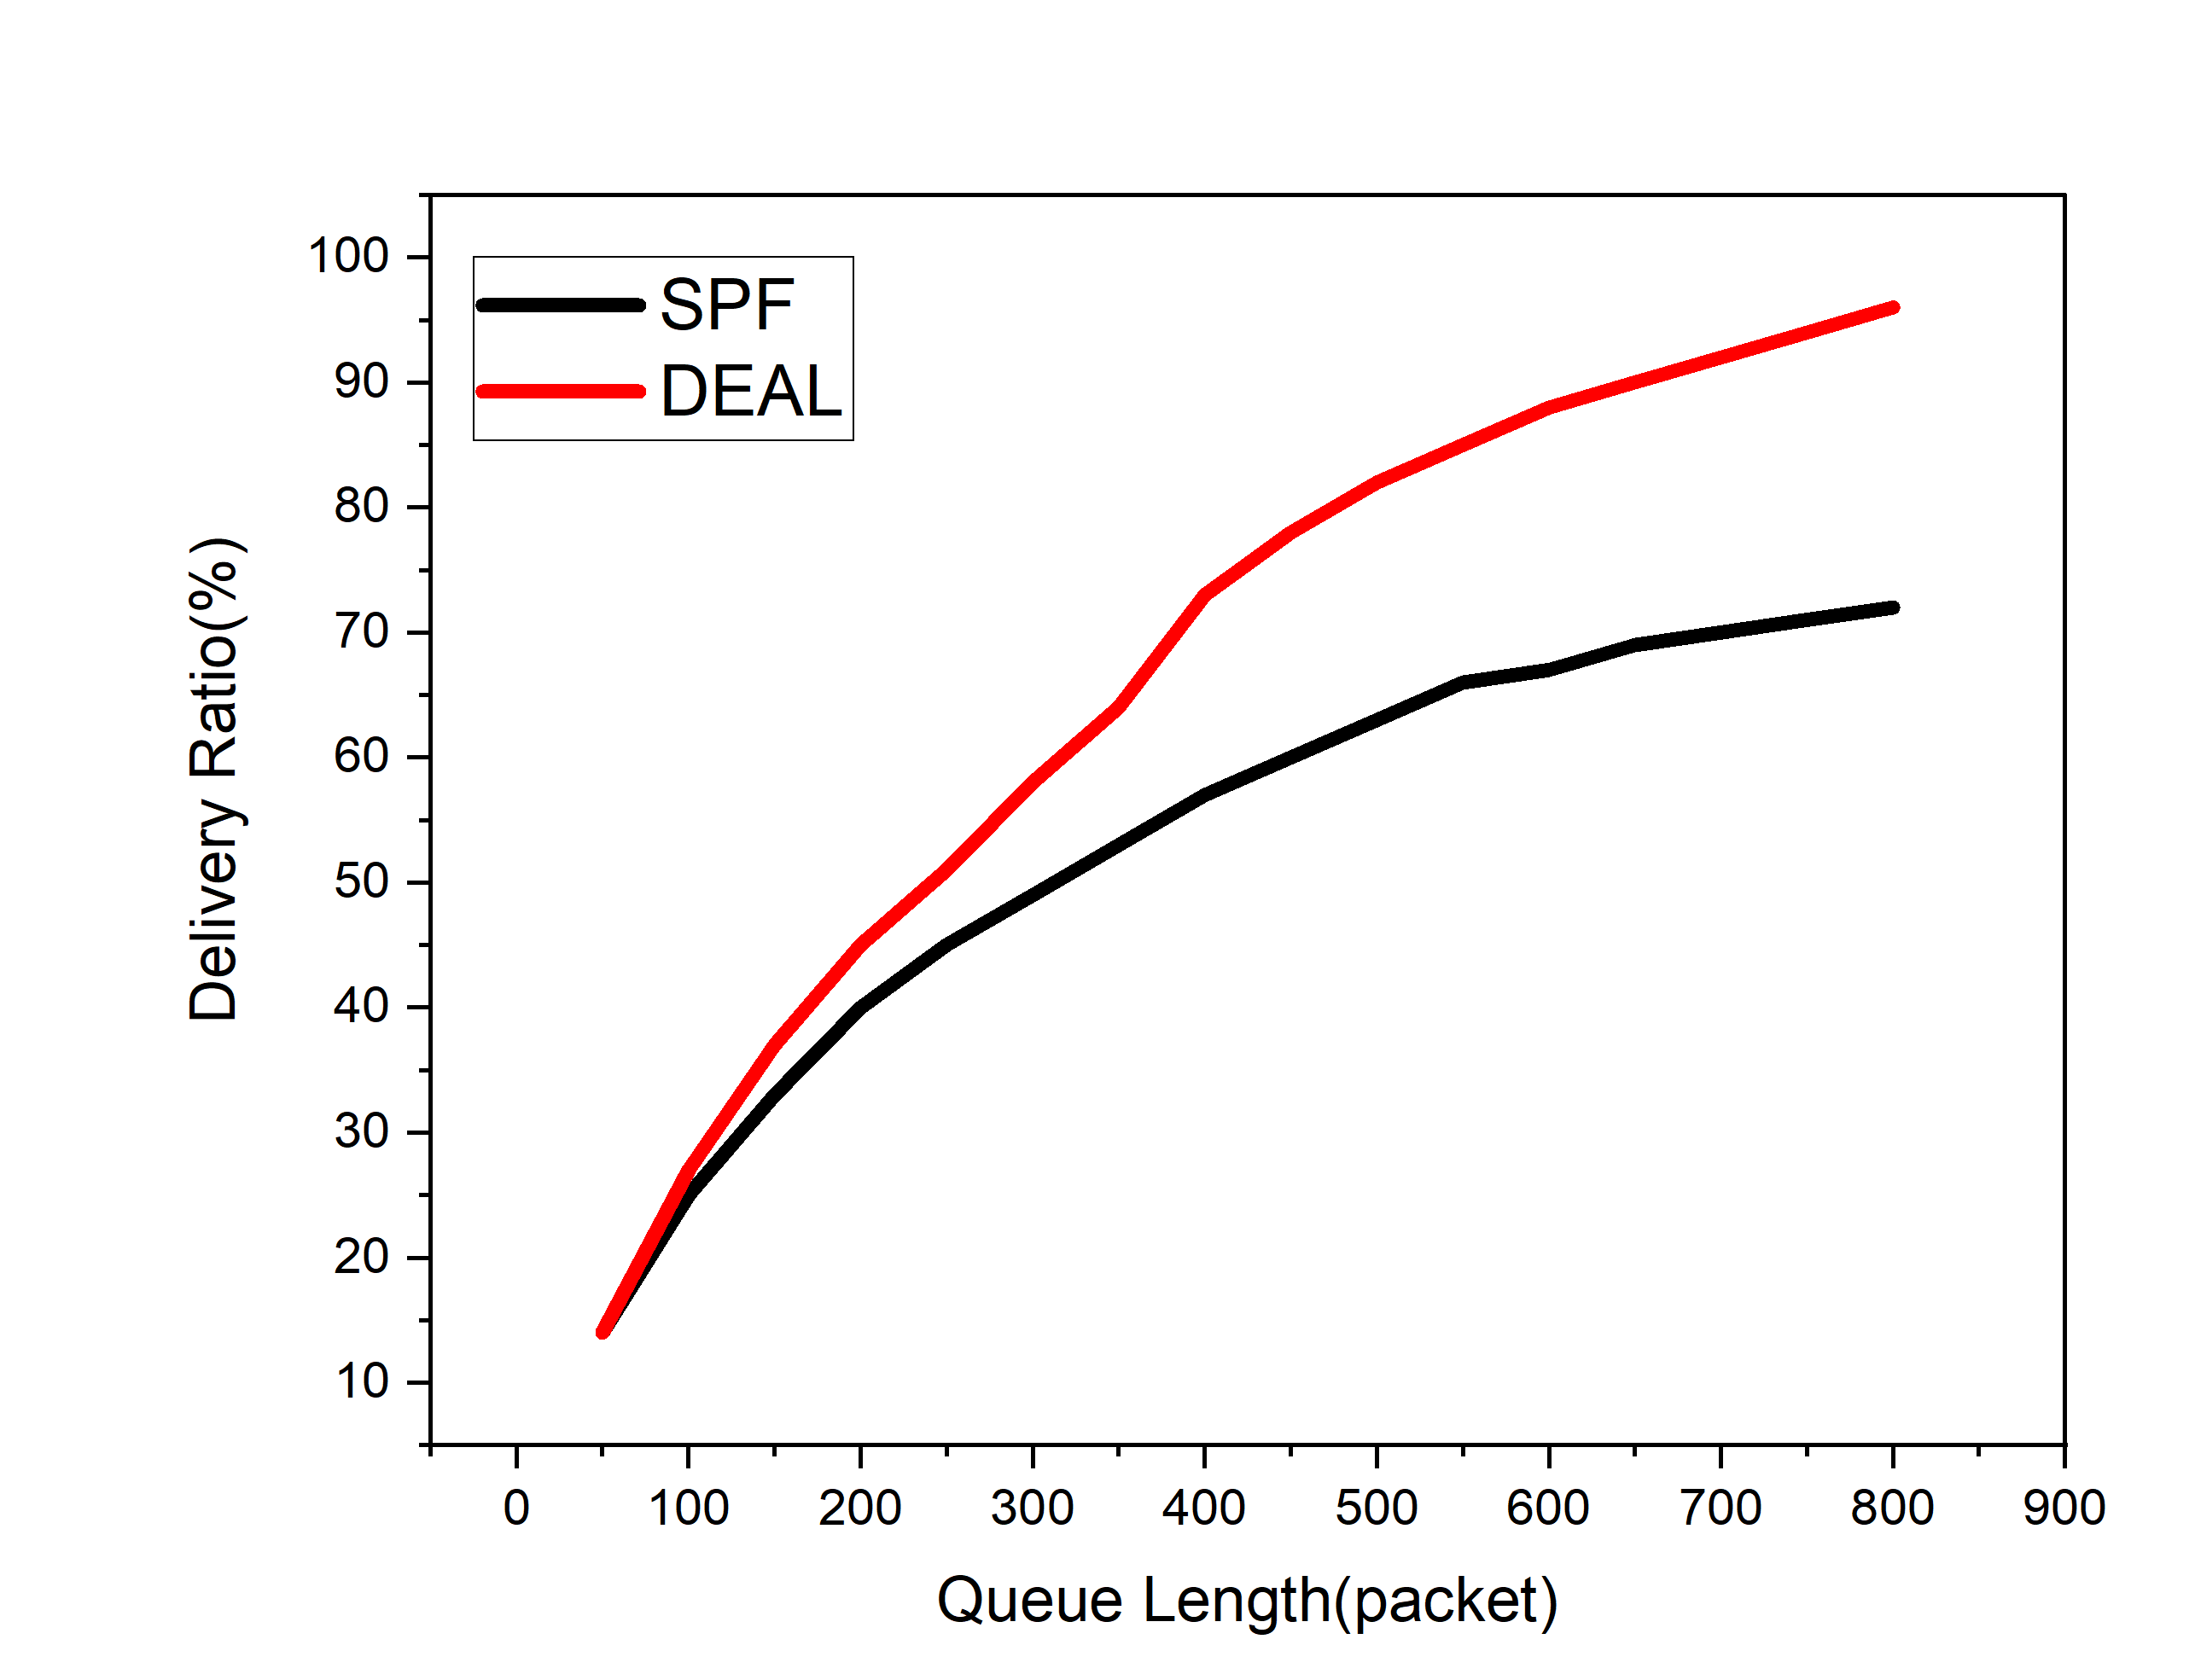
\includegraphics[width=.8\linewidth]{fig/simulation/queue/Queue-Delivery.png}
		\label{fig:QUEDELIVERY}
		}
	\subfigure[]{
		\centering
		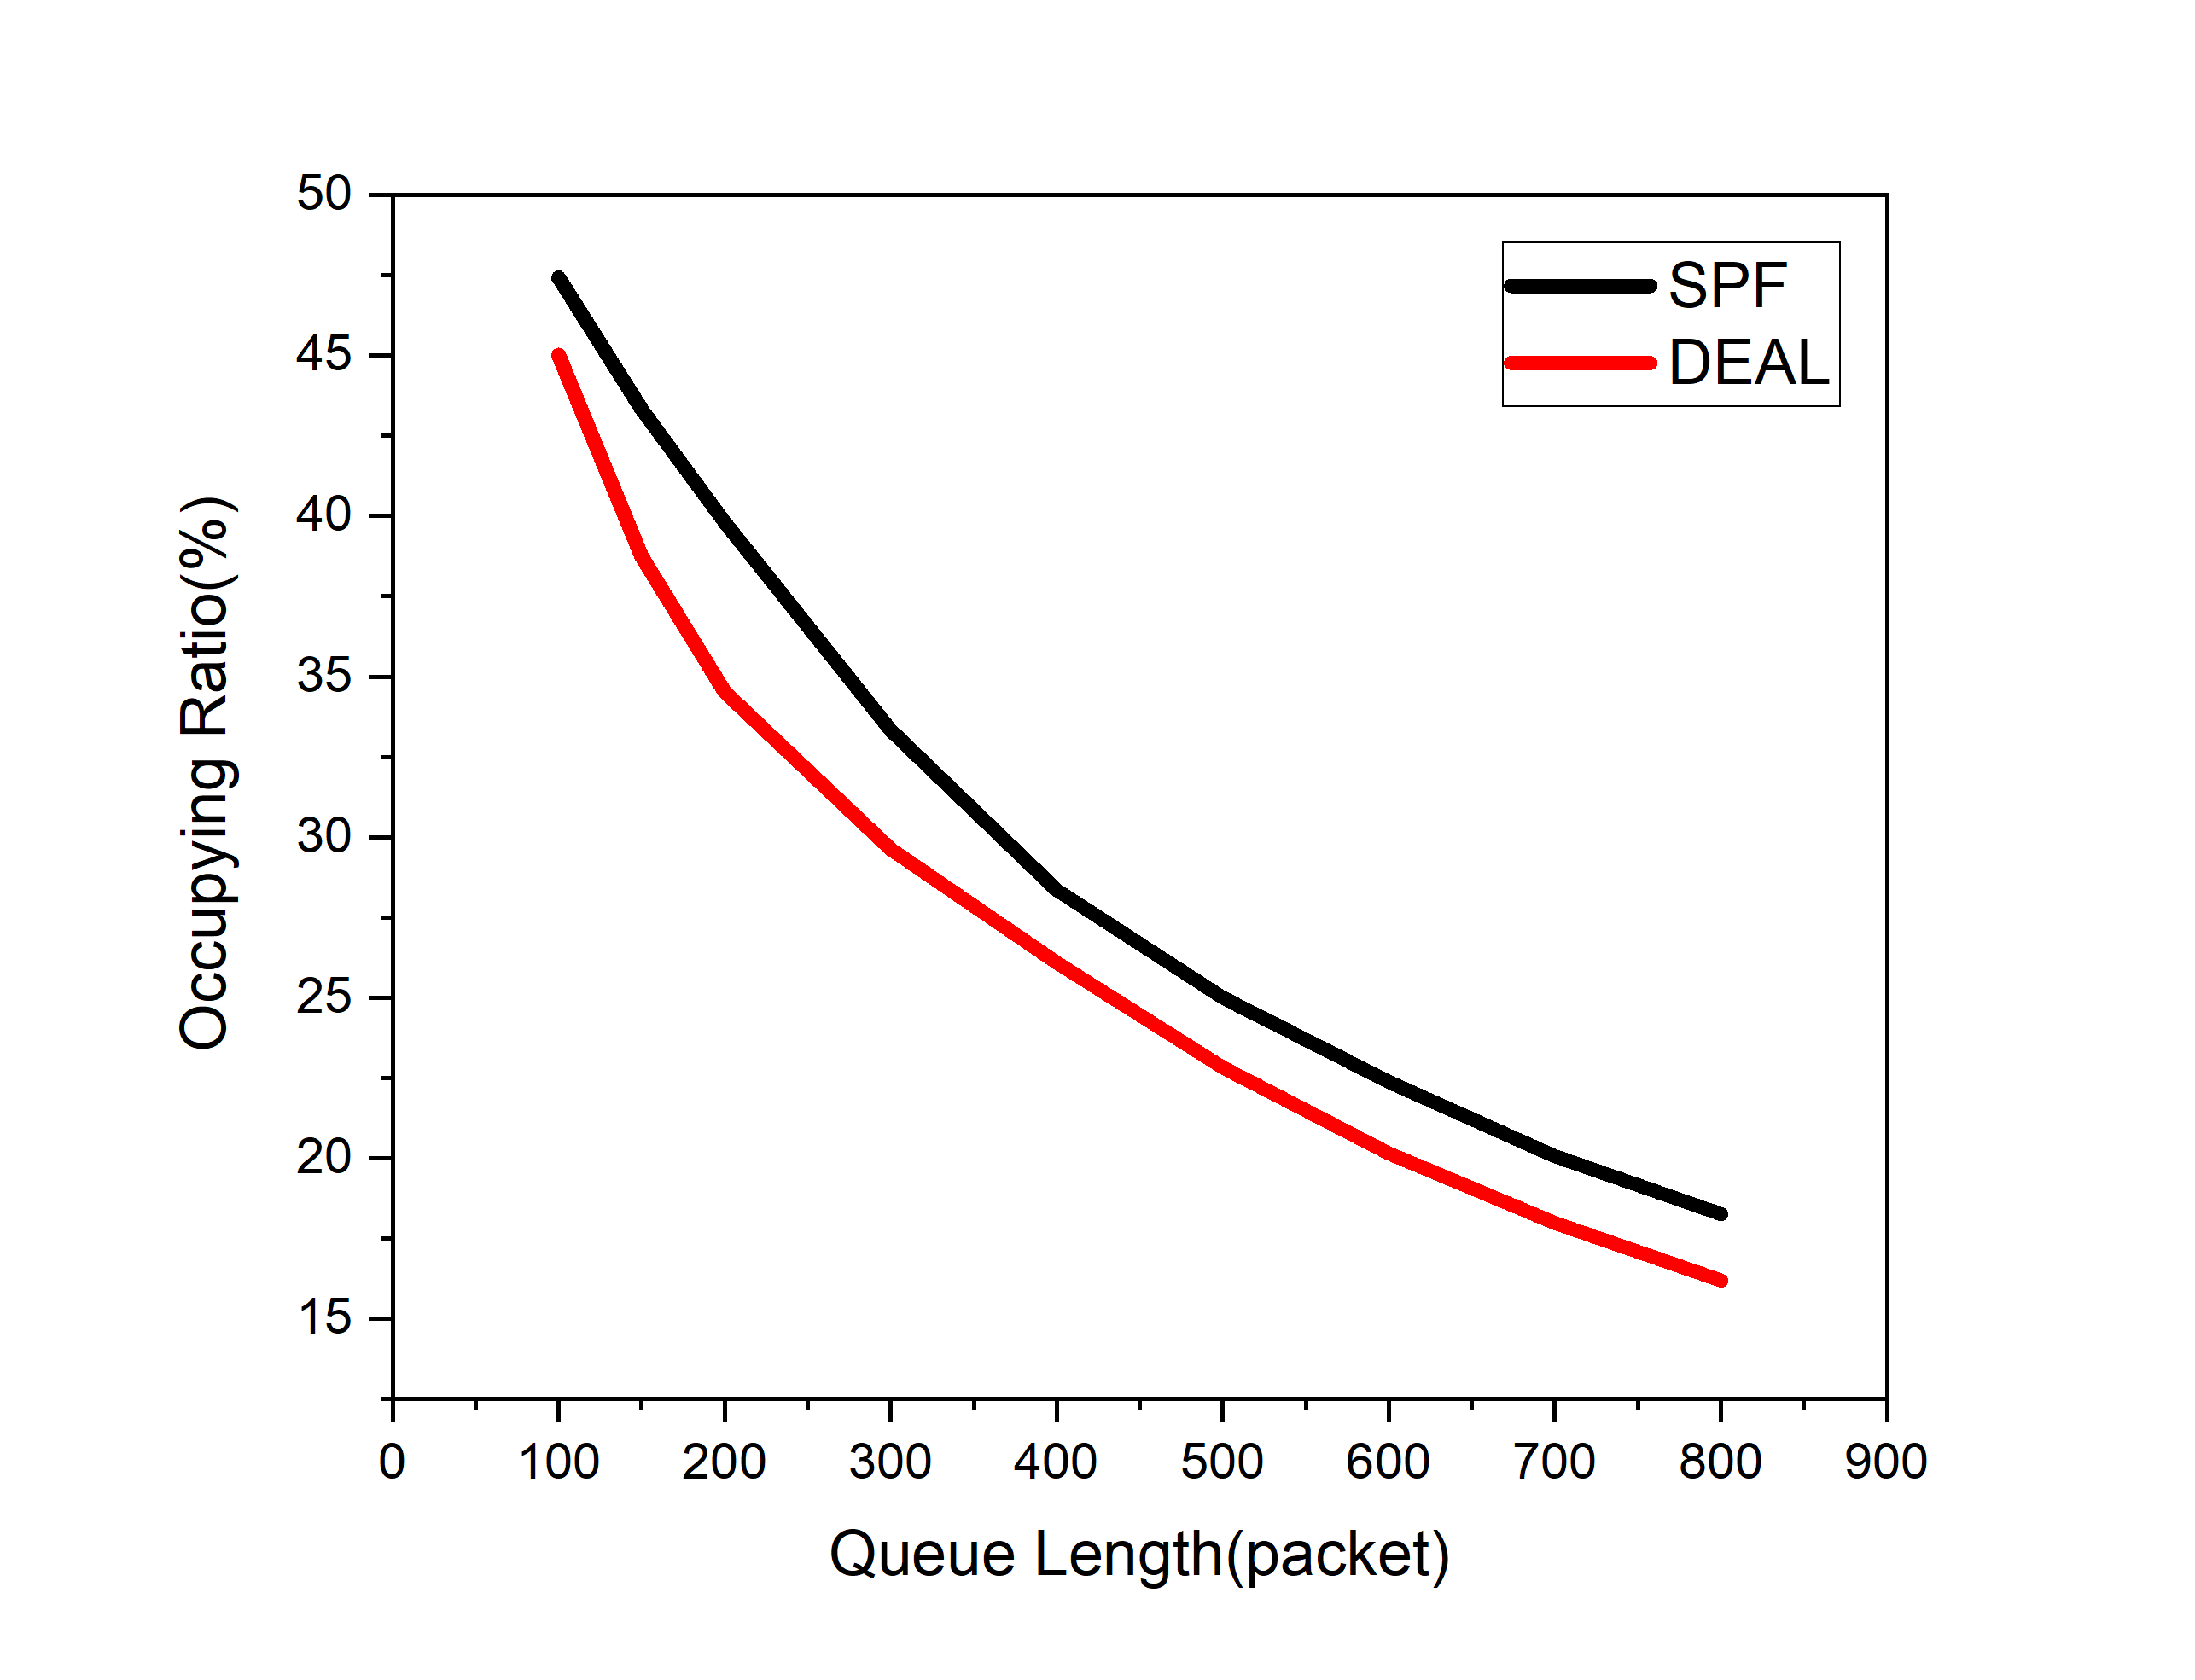
\includegraphics[width=.9\linewidth]{fig/simulation/queue/Queue-Occupying.png}
		\label{fig:QUEOCCUPYING}
		}
\caption{ (a) Delivery ratio with different buffer queue length (b) Mean Occupying ratio with different buffer queue length}
\label{fig:QUEUE}
\end{figure}

The number of dropped packets of each satellite is shown in \ref{fig:DROPPEDPACKETS}. We first labelled all the satellites as 2-digit number. The number of dropped packets in is extremely high in specific satellites because they are covering large-traffic areas, e.g. the U.S.A, China.  \ref{fig:DROPPEDPACKETSCDF} shows the CDF of dropped packets, the probability of dropped more than 40 packets is more than  10\%  in  SPF but less than 6\% in DEAL.  The performance of DEAL is better than SPF because the congestion level in  SPF is more severe. This is because our scheme  achieve a higher delivery ratio (under the same queue size) and lower the burden of queues on average. Moreover, with small queue size, the satellite in our scheme can save precious memory on satellite.
\begin{equation}
  Occupying\ Ratio\ of\ Queue :  \frac{\text { packet number in queue }}{\text { capacity of queue }} 
\end{equation}

\begin{figure}[htp]
	\subfigure[]{
		\centering
		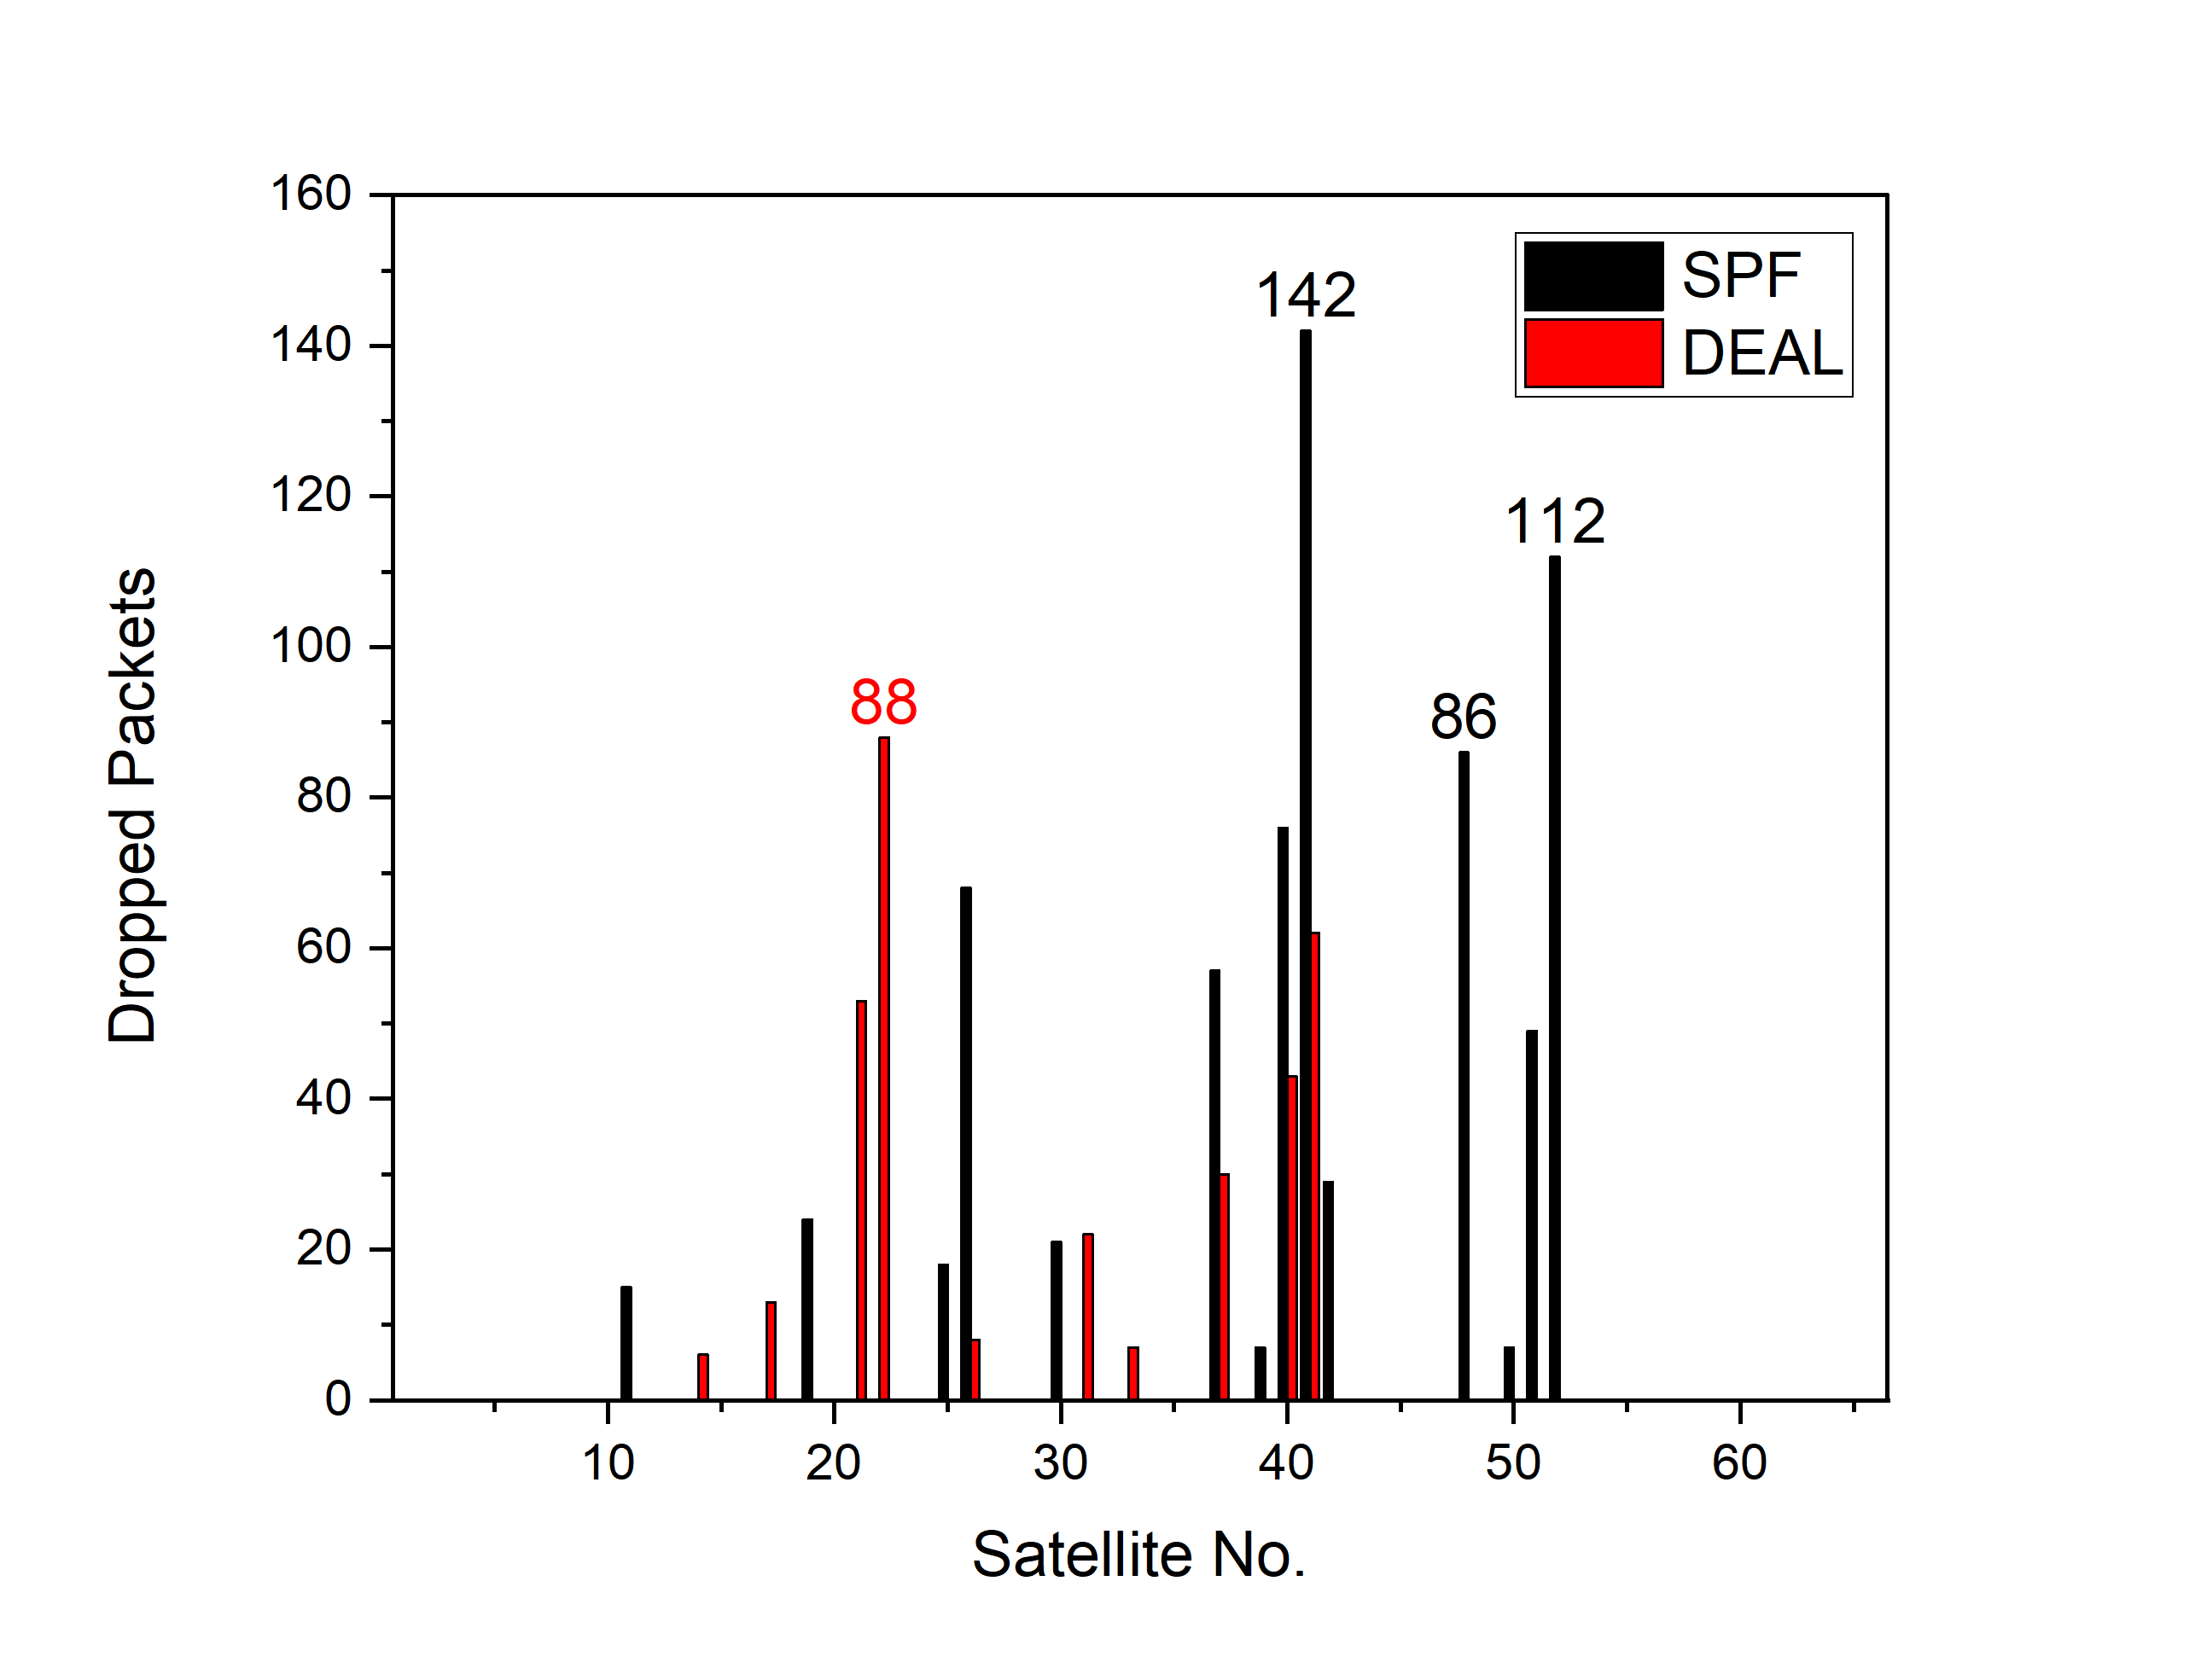
\includegraphics[width=.8\linewidth]{fig/simulation/droppedpacket/DroppedPacketsNumber.png}
		\label{fig:DROPPEDPACKETS}
		}
	\subfigure[]{
		\centering
		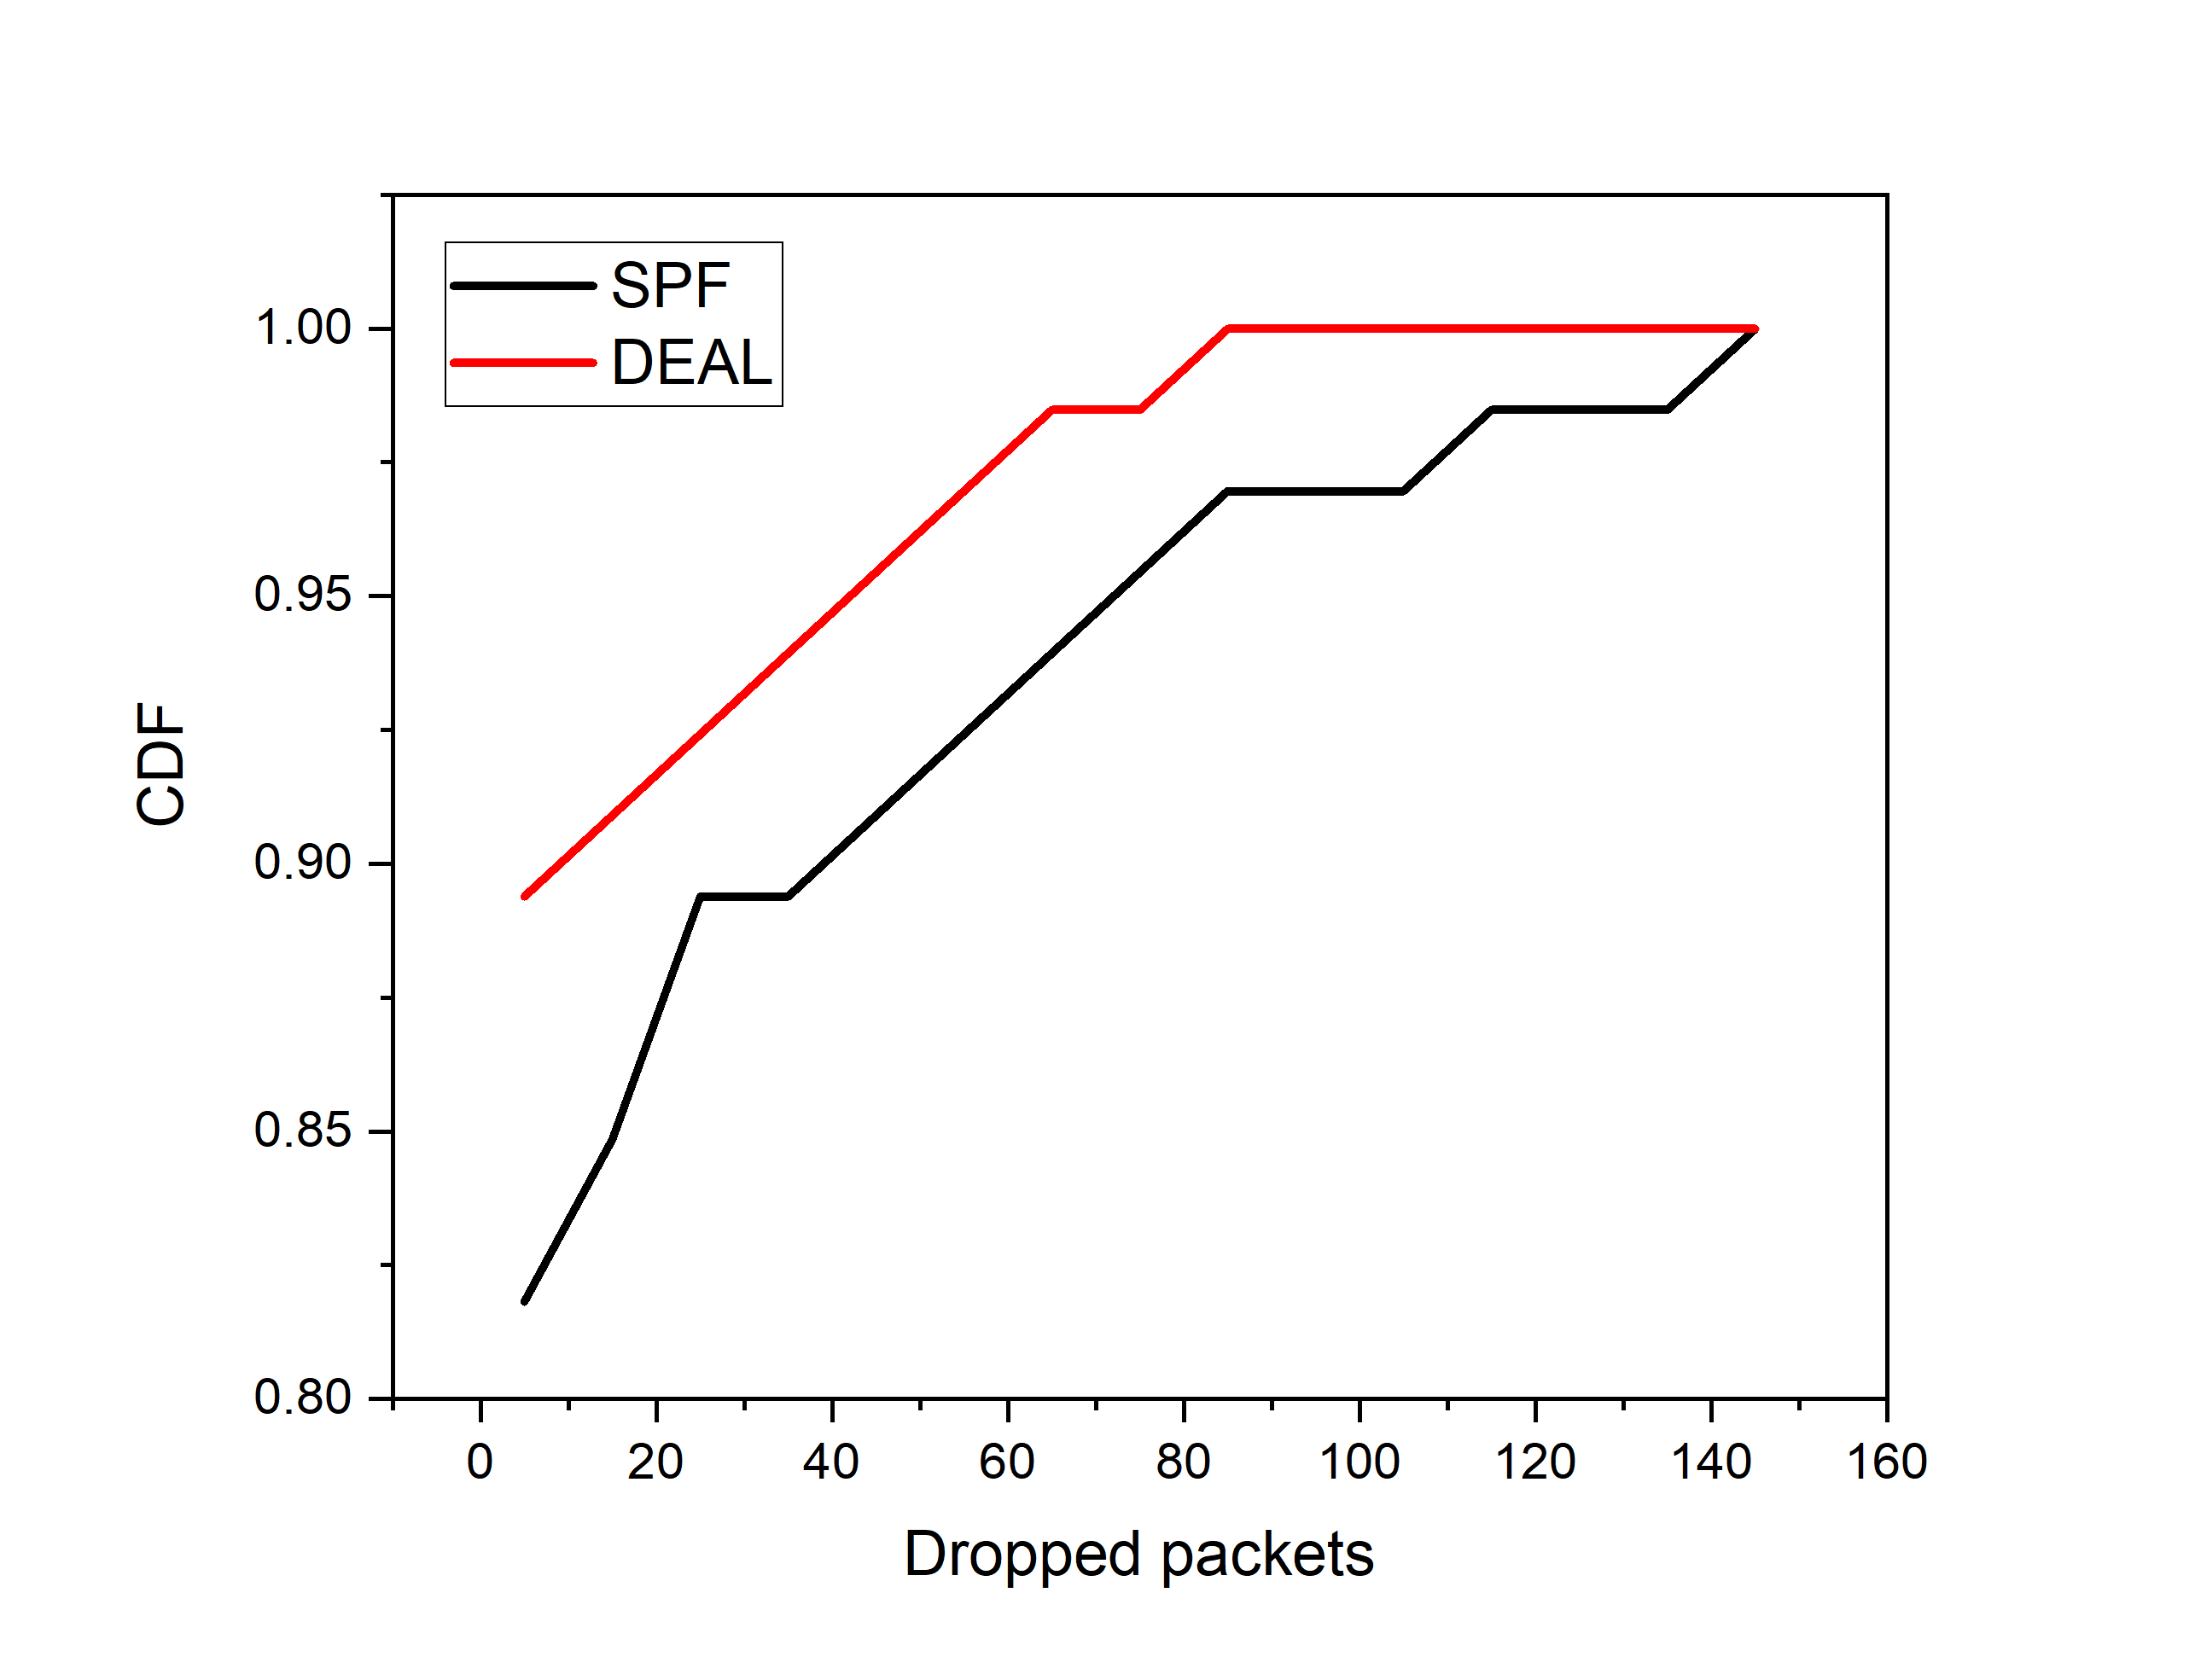
\includegraphics[width=.8\linewidth]{fig/simulation/droppedpacket/DroppedPacketsCDF.png}
		\label{fig:DROPPEDPACKETSCDF}
		}
\caption{ (a) Dropped packets of each satellite (b) CDF of dropped packets}
\label{fig:DROPPED}
\end{figure}

Below in order to compare the link utilization, end-to-end delay, and remaining battery of two schemes under the same delivery ratio.  We set the higher channel data rate and larger queue size as 15Mbps and 650 packet length. When the delivery ratios of the two schemes are different, the impact of undelivered packets can  not be evaluated fairly.


\subsection{Impact of Battery}
At first, we compare the remaining battery energy of the two schemes. In \ref{fig:SPFENERGY} and  \ref{fig:DEALENERGY}, the remaining energy of each satellite's battery in SPF is more diverse than that of DEAL. The standard deviation of remaining energy in SPF is 1127.5, and the standard deviation of remaining energy in DEAL is 1020.76. Besides, the minimal remaining energy of SPF, 30.9,  is much smaller than that of DEAL, 59.2, which indicates that the DEAL algorithm outperforms the SPF algorithm bases its routing strategy on only finding one path.  \ref{fig:CDFENERGY} shows the remaining energy CDF of two schemes. Then we can see DEAL can perform better in energy average for satellite networks.

\begin{figure}[htp]
	\centering
	\subfigure[]{
		\centering
		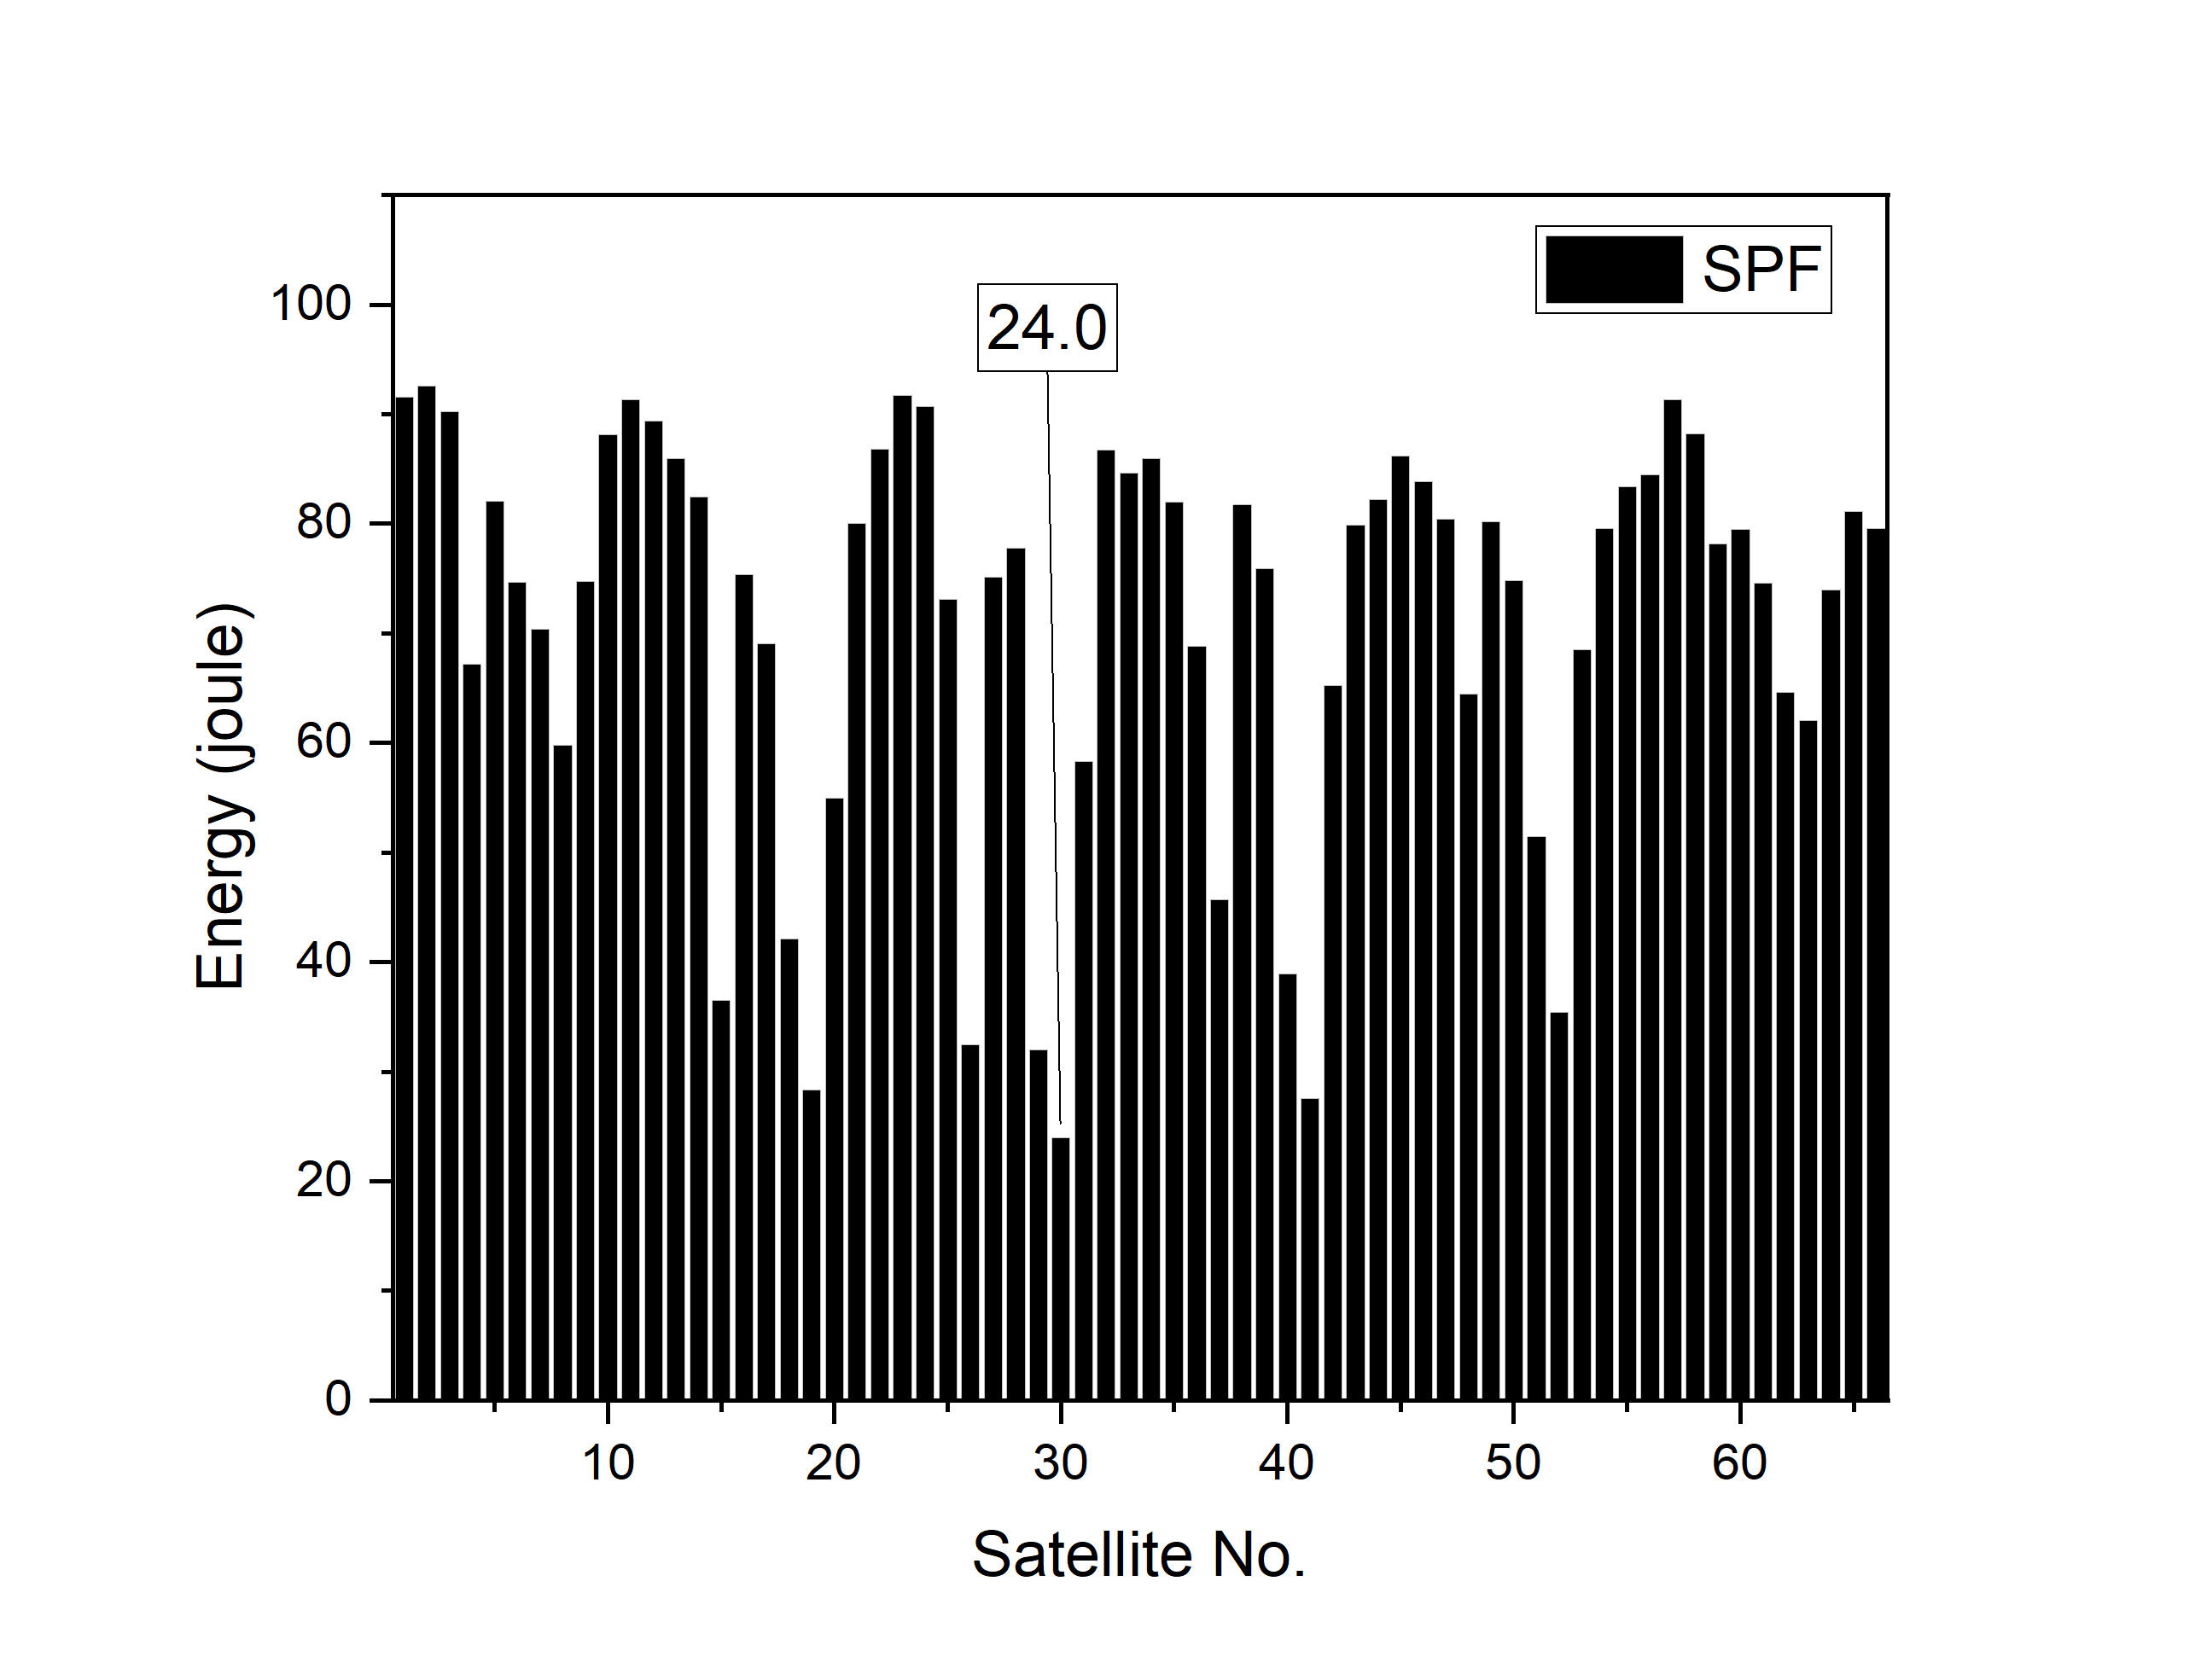
\includegraphics[width=.8\linewidth]{fig/simulation/energy/SPF-ENERGY.png}
		\label{fig:SPFENERGY}
		}
	\subfigure[]{
		\centering
		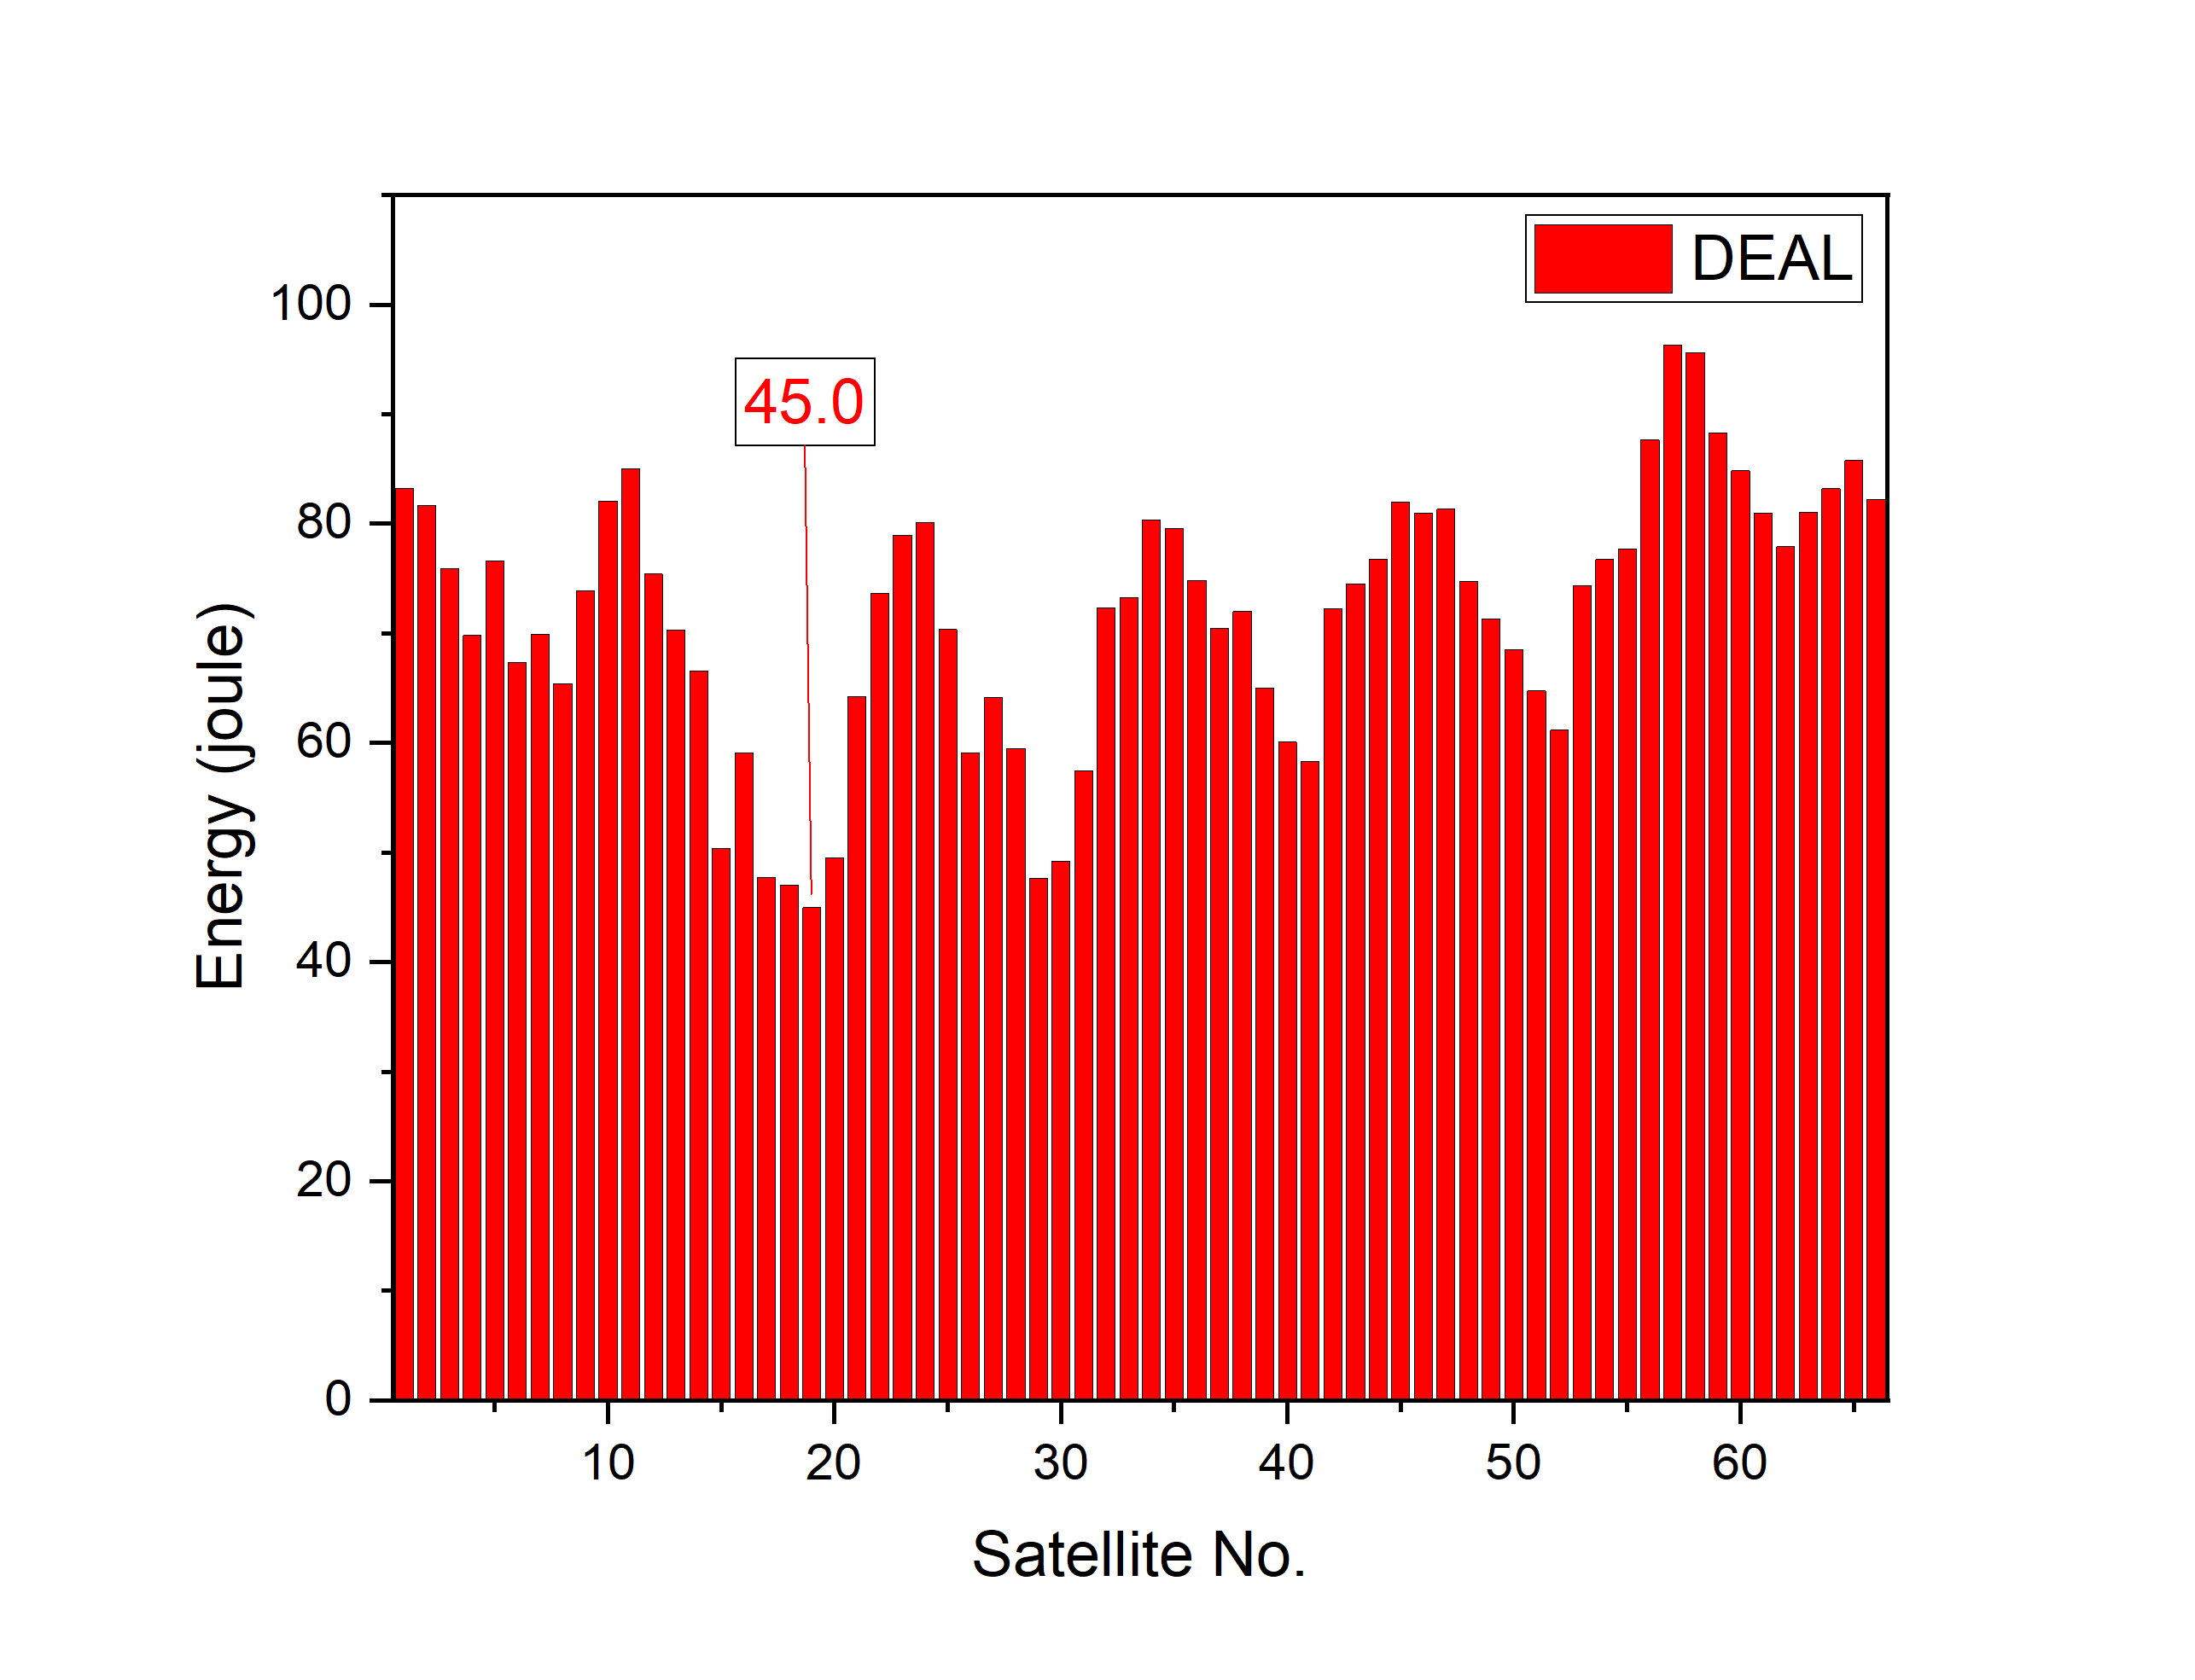
\includegraphics[width=.8\linewidth]{fig/simulation/energy/DEAL-ENERGY.png}
		\label{fig:DEALENERGY}
		}
	\subfigure[]{
		\centering
		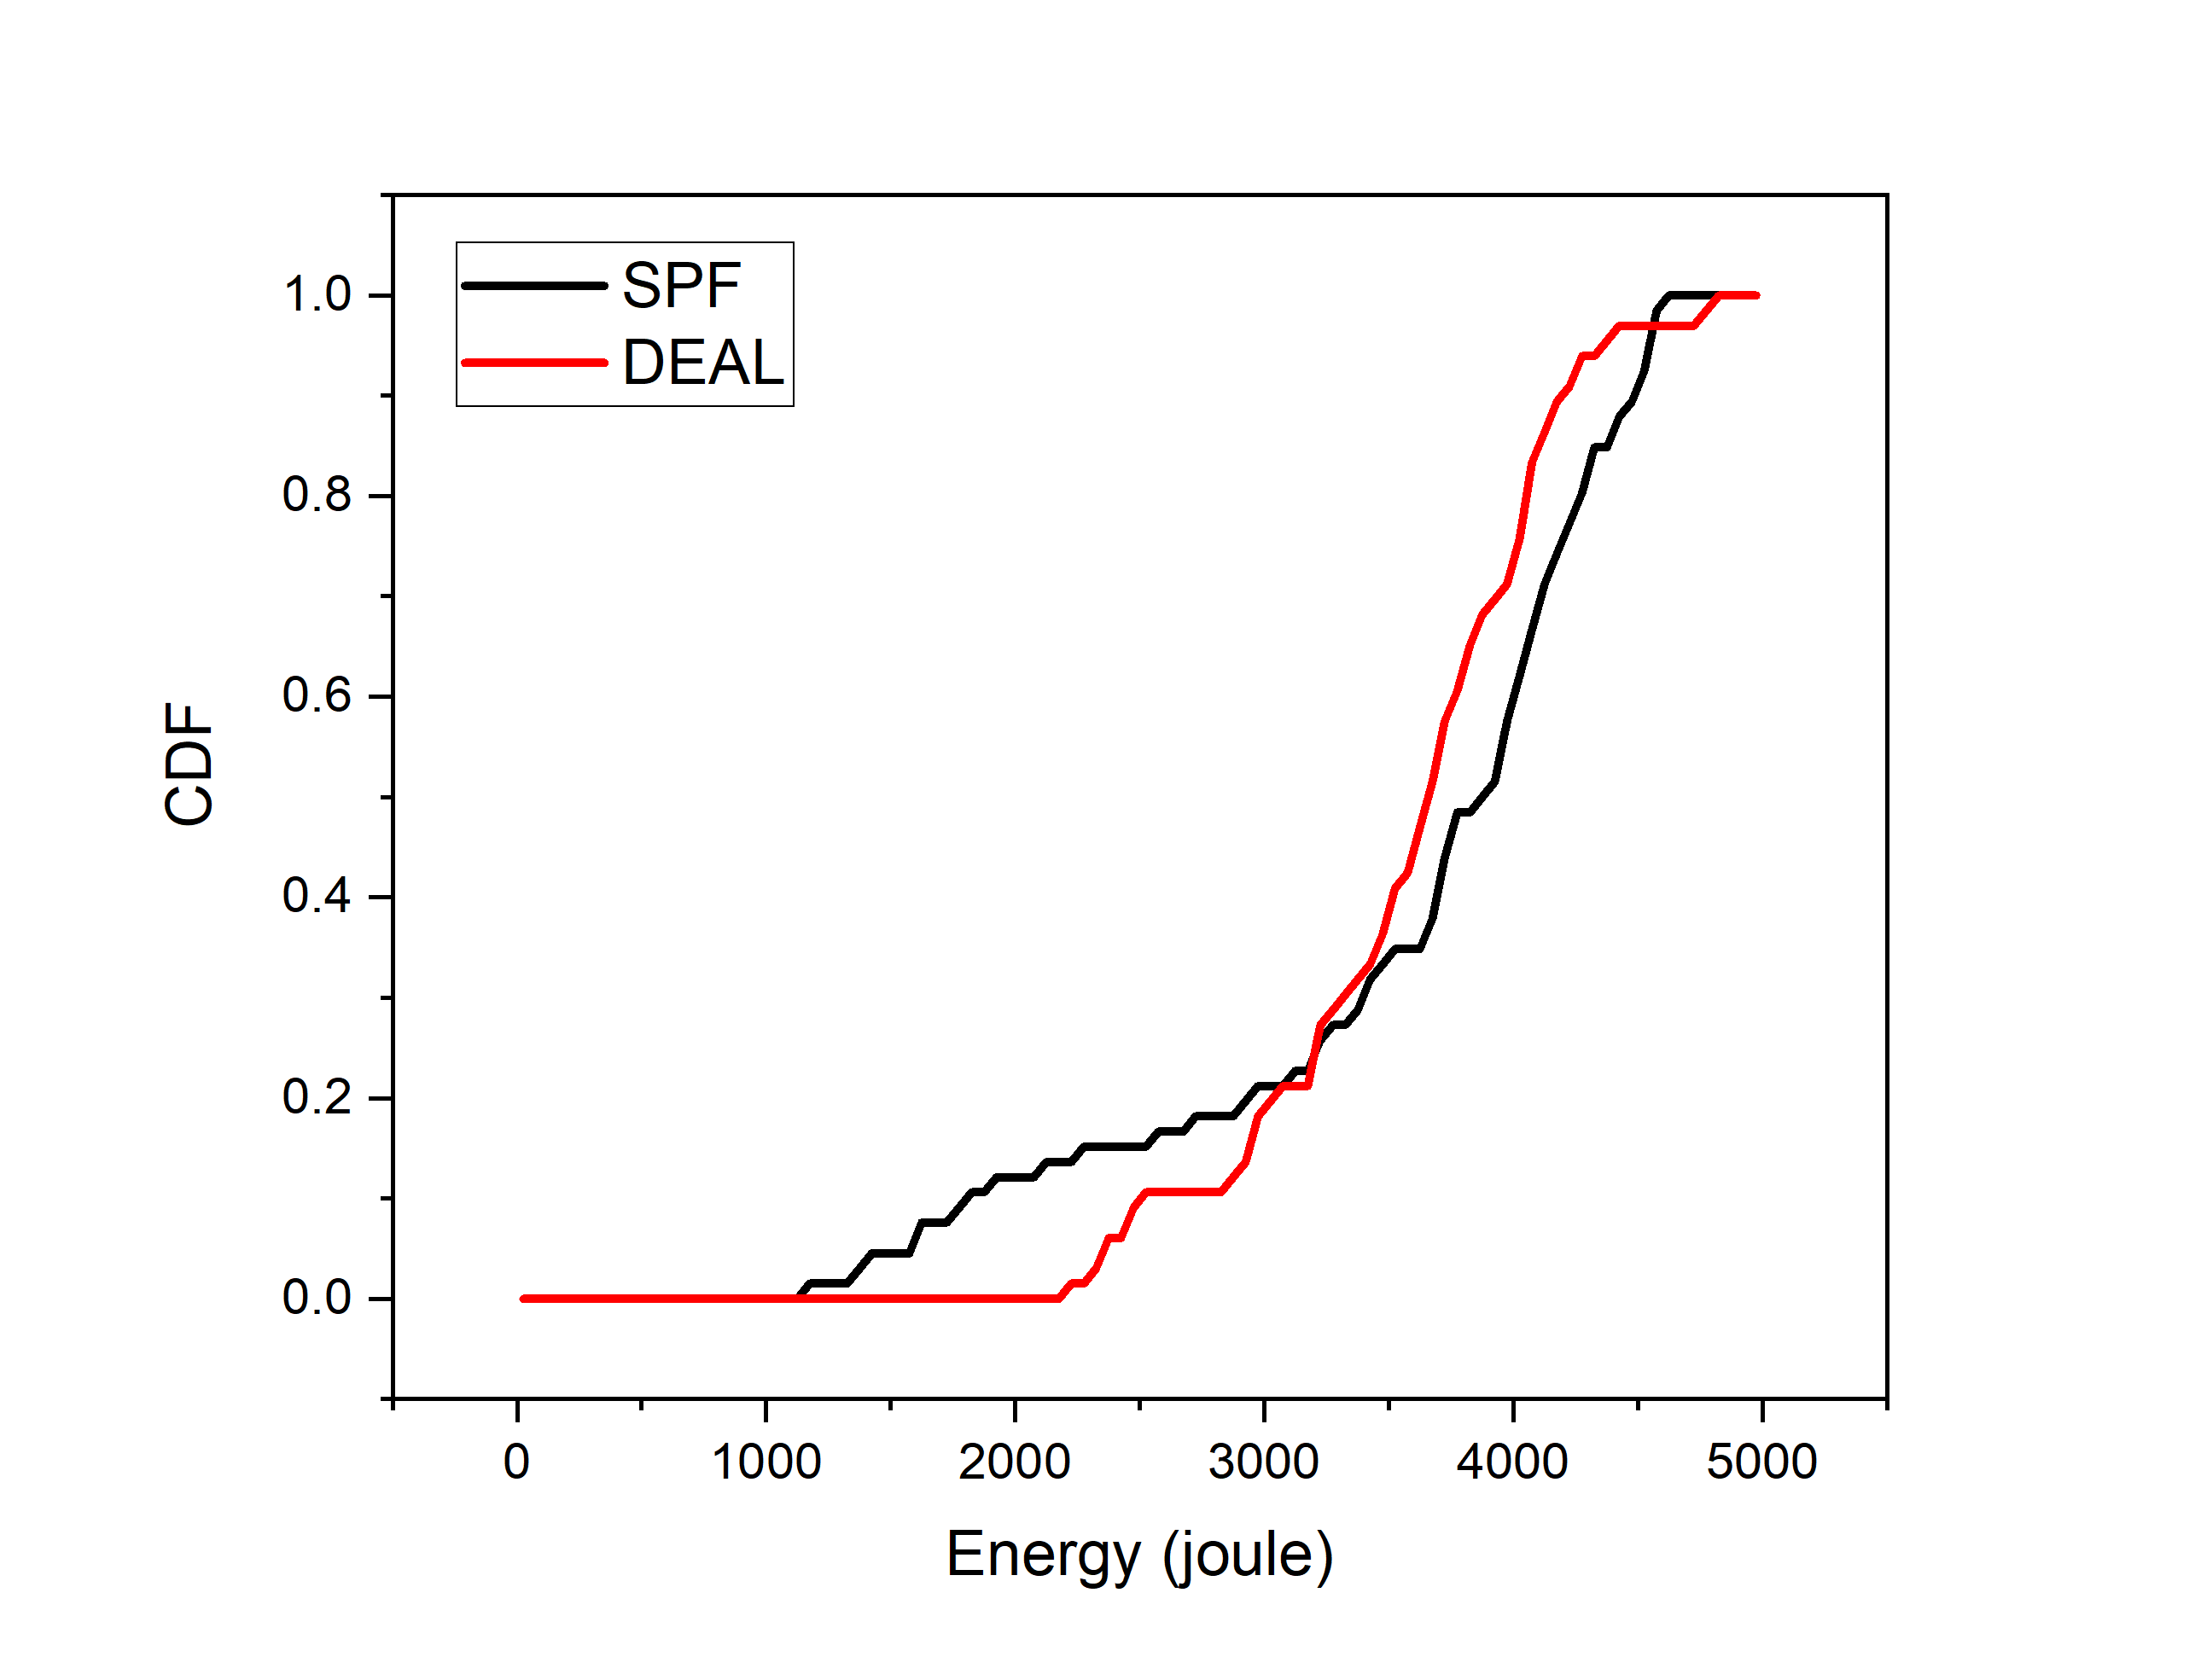
\includegraphics[width=.8\linewidth]{fig/simulation/energy/CDF-ENERGY.png}
		\label{fig:CDFENERGY}
		}
\caption{ (a) Remaining energy of each satellite in SPF (b)  Remaining energy of each satellite in DEAL (c) CDF of remaining energy}
\label{fig:ENERGY}
\end{figure}

\subsection{Impact of Link Utilization}
\ref{fig:LU} shows the link utilization. All the links in satellite constellation are labelled as 3-digit number. Compared to SPF, our DEAL has smaller link utilization, most link has utilization lower than 25\%. Moreover, SPF's mean link utilization is about 0.080202, while DEAL's mean value of link utilization is about 0.0731. The standard deviation of SPF is 0.06606, and DEAL's is 0.0549, and the CDF of link utilization is shown in \ref{fig:LUCDF}. The highest link utilization in SPF is 32.76563, while the highest one in DEAL is 27.5531. This is because DEAL splits the flows and reduces the possiblity of congestion.

\begin{figure}[htp]
	\subfigure[]{
		\centering
		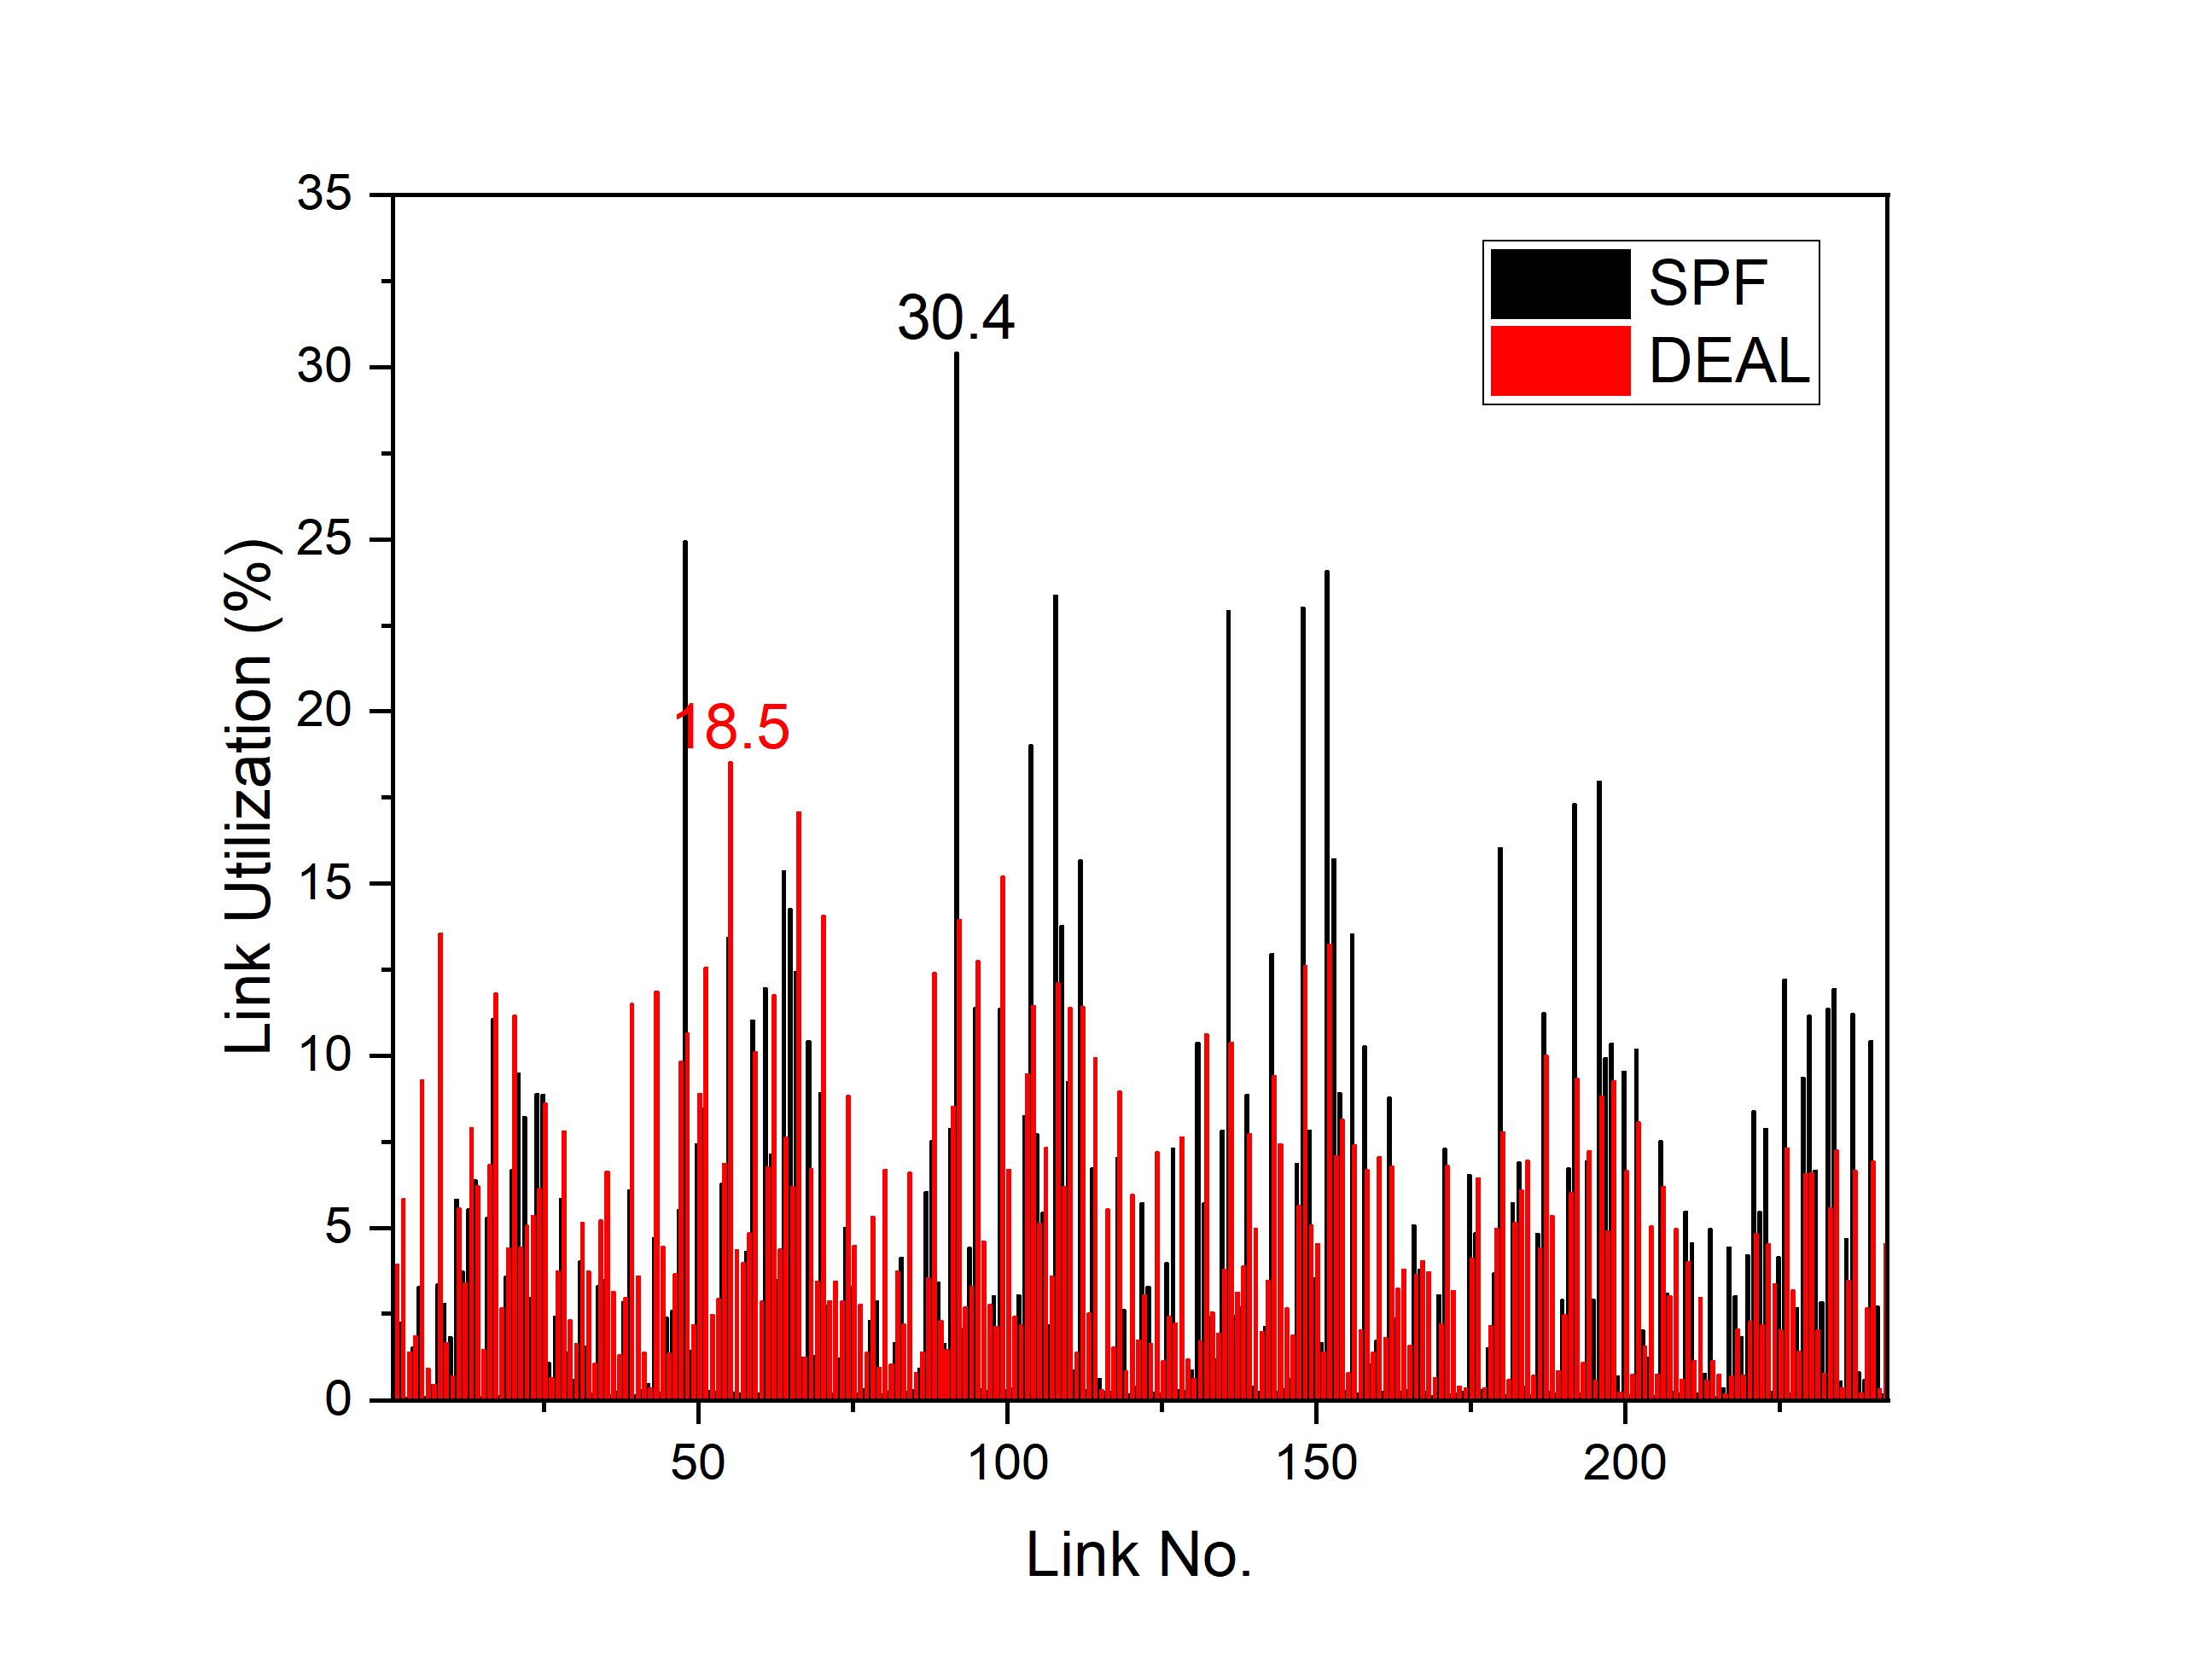
\includegraphics[width=.8\linewidth]{fig/simulation/linkUtilization/LinkUtilization.png}
		\label{fig:LU}
		}
	\subfigure[]{
		\centering
		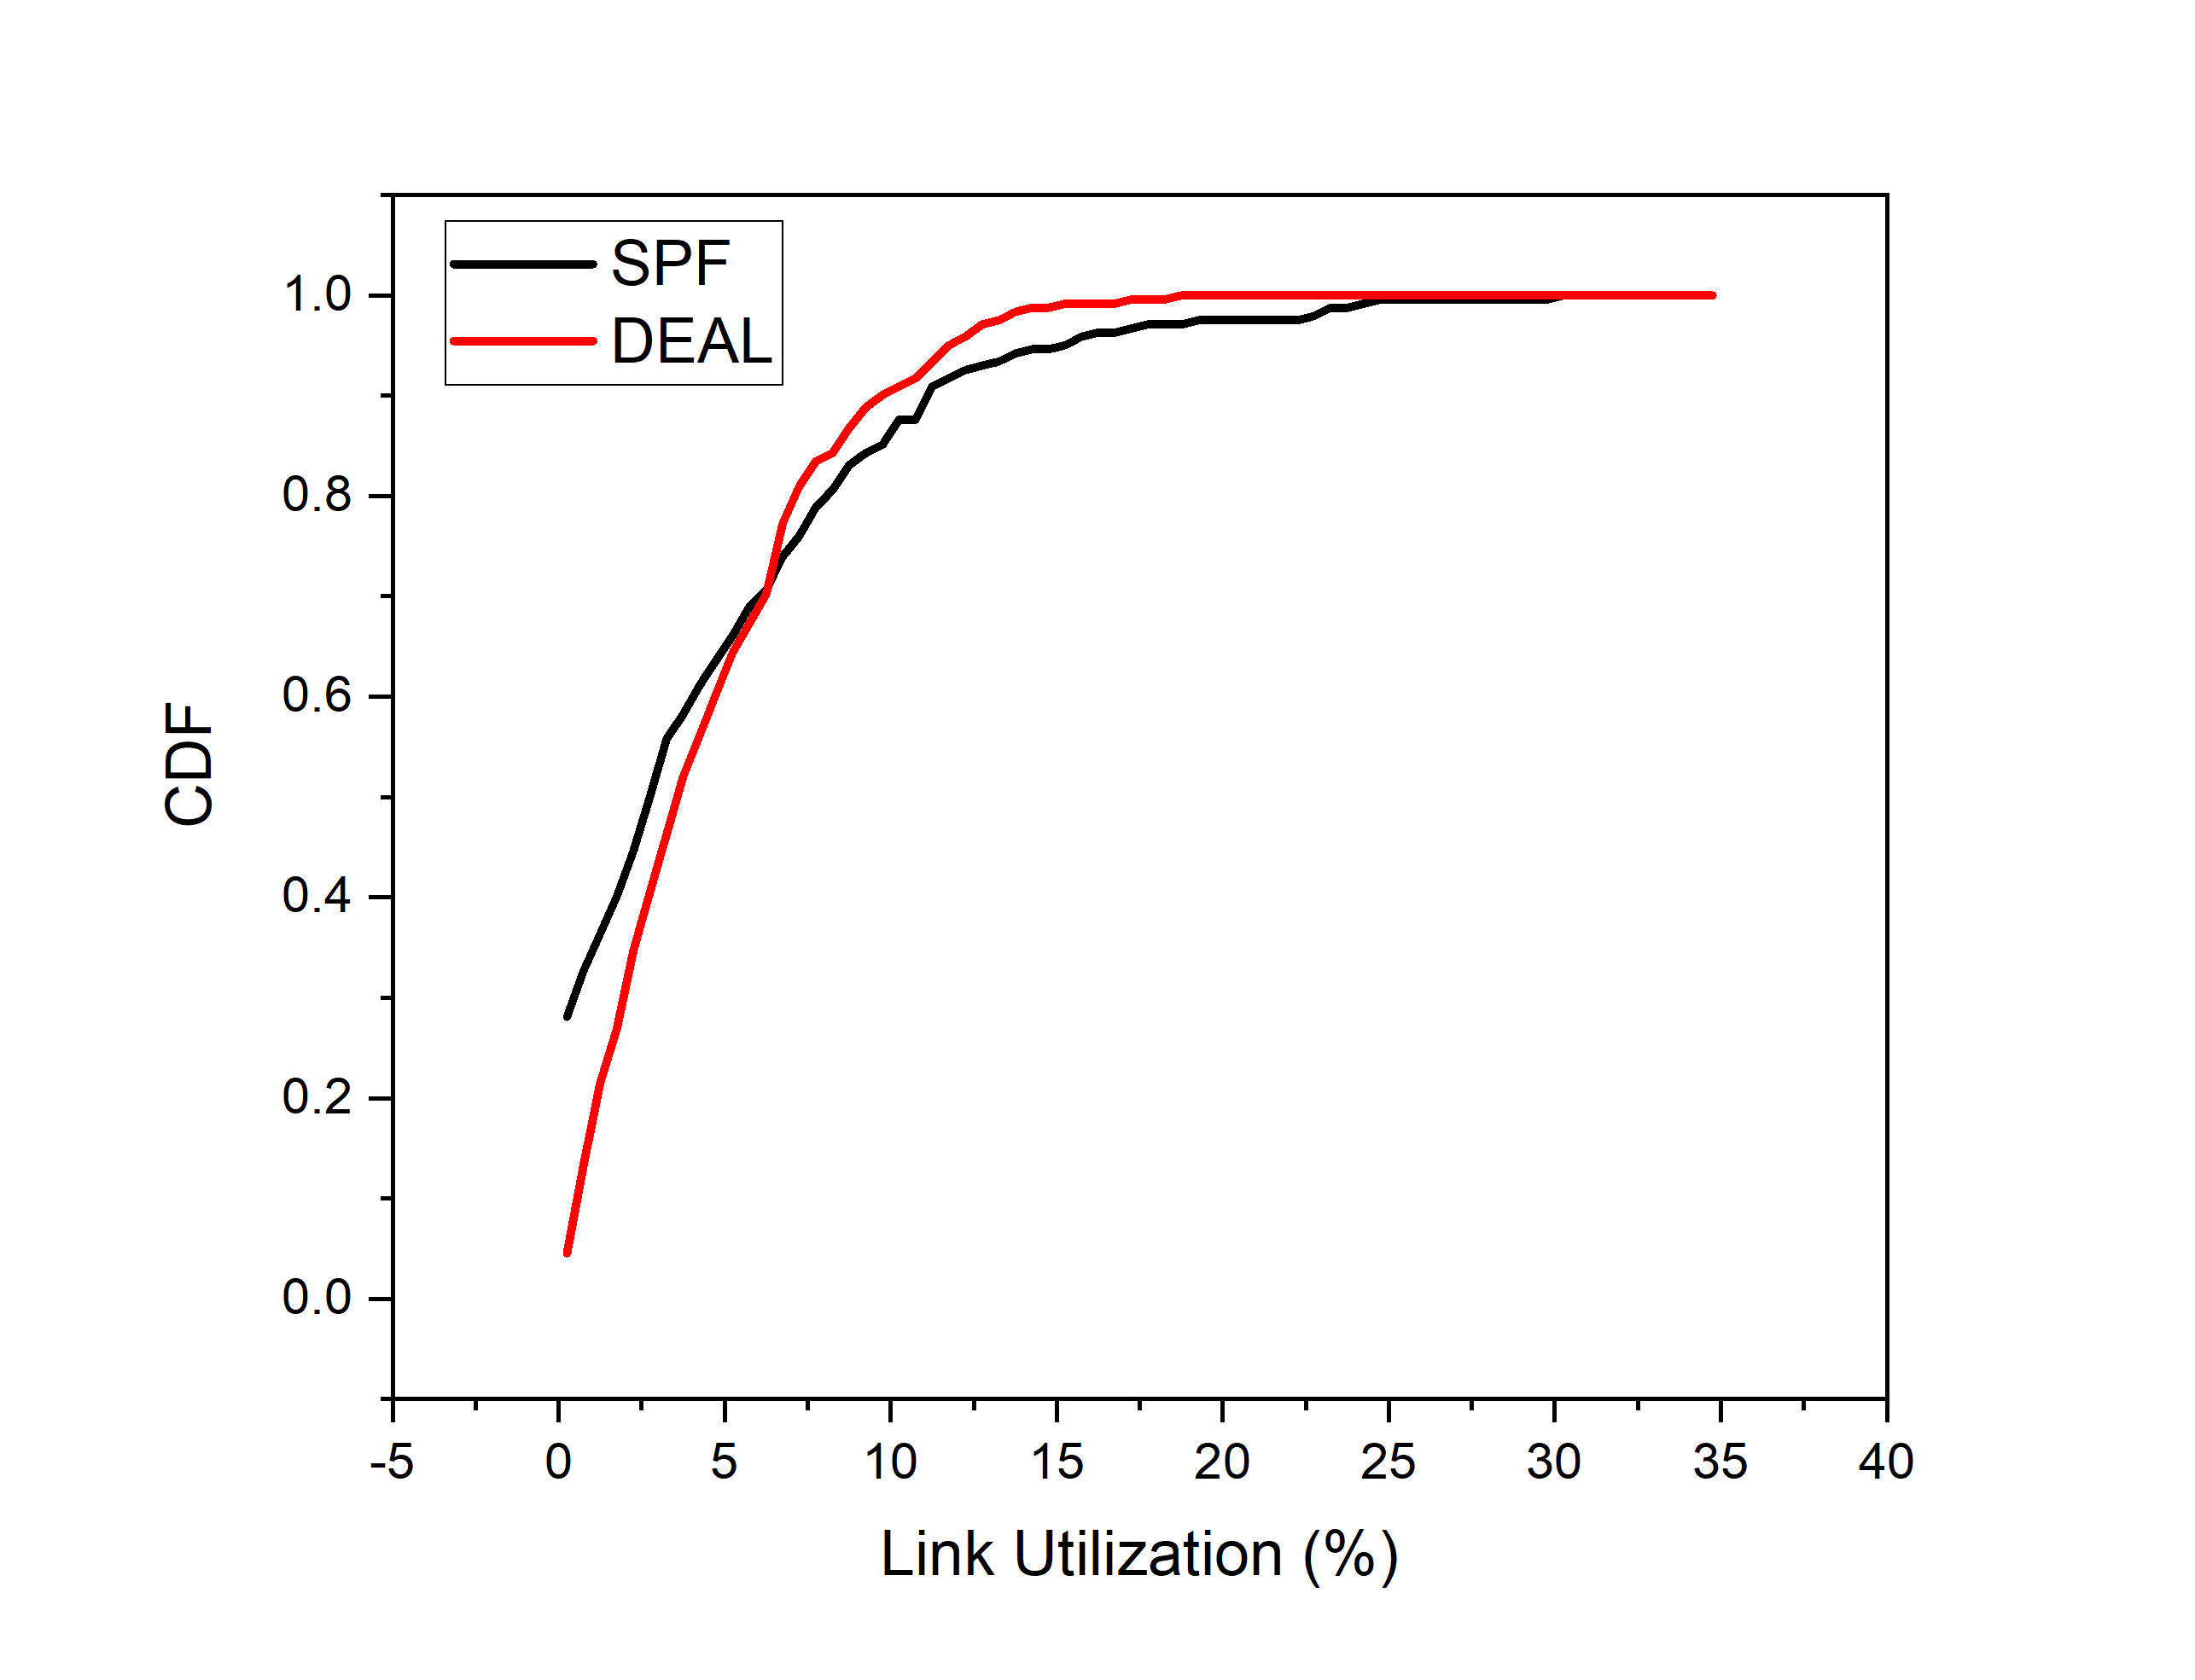
\includegraphics[width=.8\linewidth]{fig/simulation/linkUtilization/LinkUtilizationCDF.png}
		\label{fig:LUCDF}
		}
	
\caption{(a) Link utilization of each link (b) CDF of link Utilization}
\label{fig:UTILIZATION}
\end{figure}


\subsection{Impact of End-to-End Delay }

The mean end-to-end delay of a satellite is the average delay of packets of the same communication satellite pair. In our simulation, the mean delay of a packet in SPF is about 0.153ms, and the mean delay of a packet in DEAL is about 0.136ms. The mean delay of each satellite is presented in \ref{fig:ENDTOENDDELAY}. in which the average delay is calculated and presented.  The two schemes have a slight difference which comes from the queuing delay.

\begin{figure}[htp]
	\centering
	
	\subfigure[]{
		\centering
		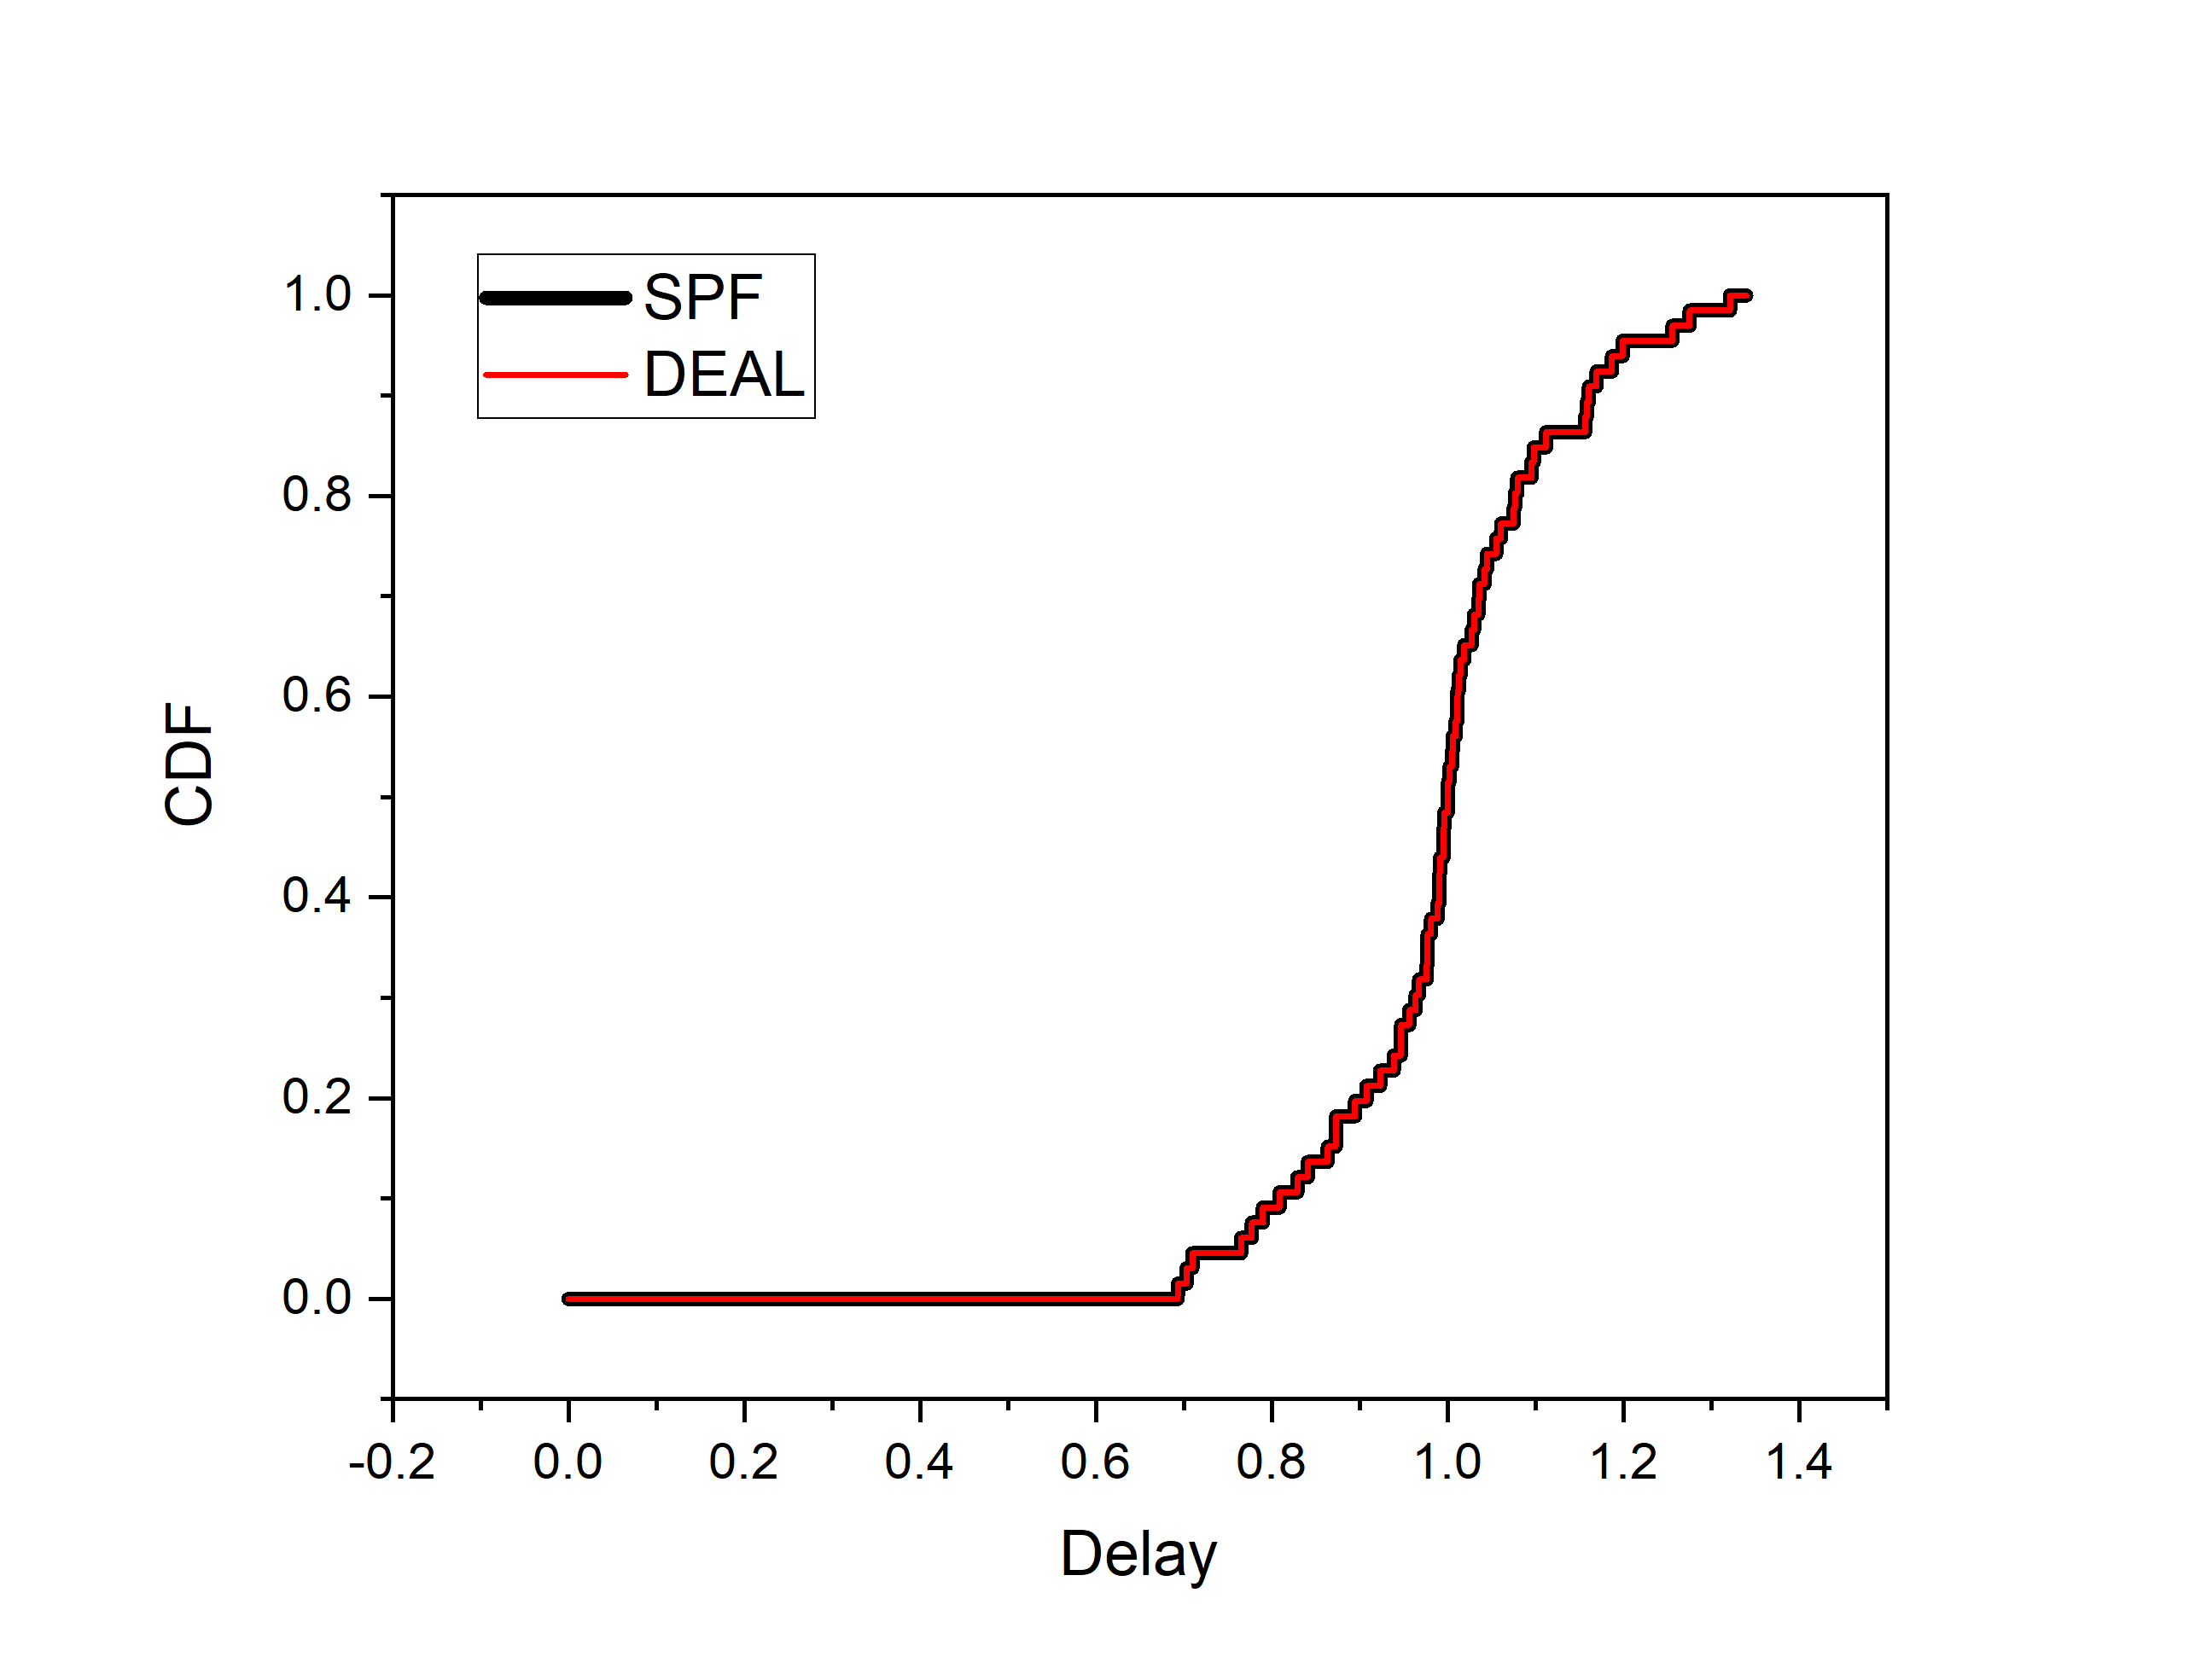
\includegraphics[width=.8\linewidth]{fig/simulation/delay/ENDTOENDDELAY.png}
		\label{fig:ENDTOENDDELAY}
		}
	
\caption{CDF of Mean End-to-End Delay}
\label{fig:DELAY}
\end{figure}

To show the probability of congestion, we  compare their mean occupying ratio of buffer queues. In \ref{fig:ORES} and \ref{fig:CDFOR}, several satellites in SPF has rather high occupying ratio of the queue. Recall that packets with a given source satellite and destination satellite adopt the same route in SPF, and some satellites became hot-spots. Clearly, congestion happens easily when satellites on the paths cover the high-population area.  DEAL adopts flow splitting to avoid the congestion with different cost value along with distance, the probability of congestion in DEAL can be lower. 

\begin{figure}[htp]
	\centering
	\subfigure[]{
		\centering
		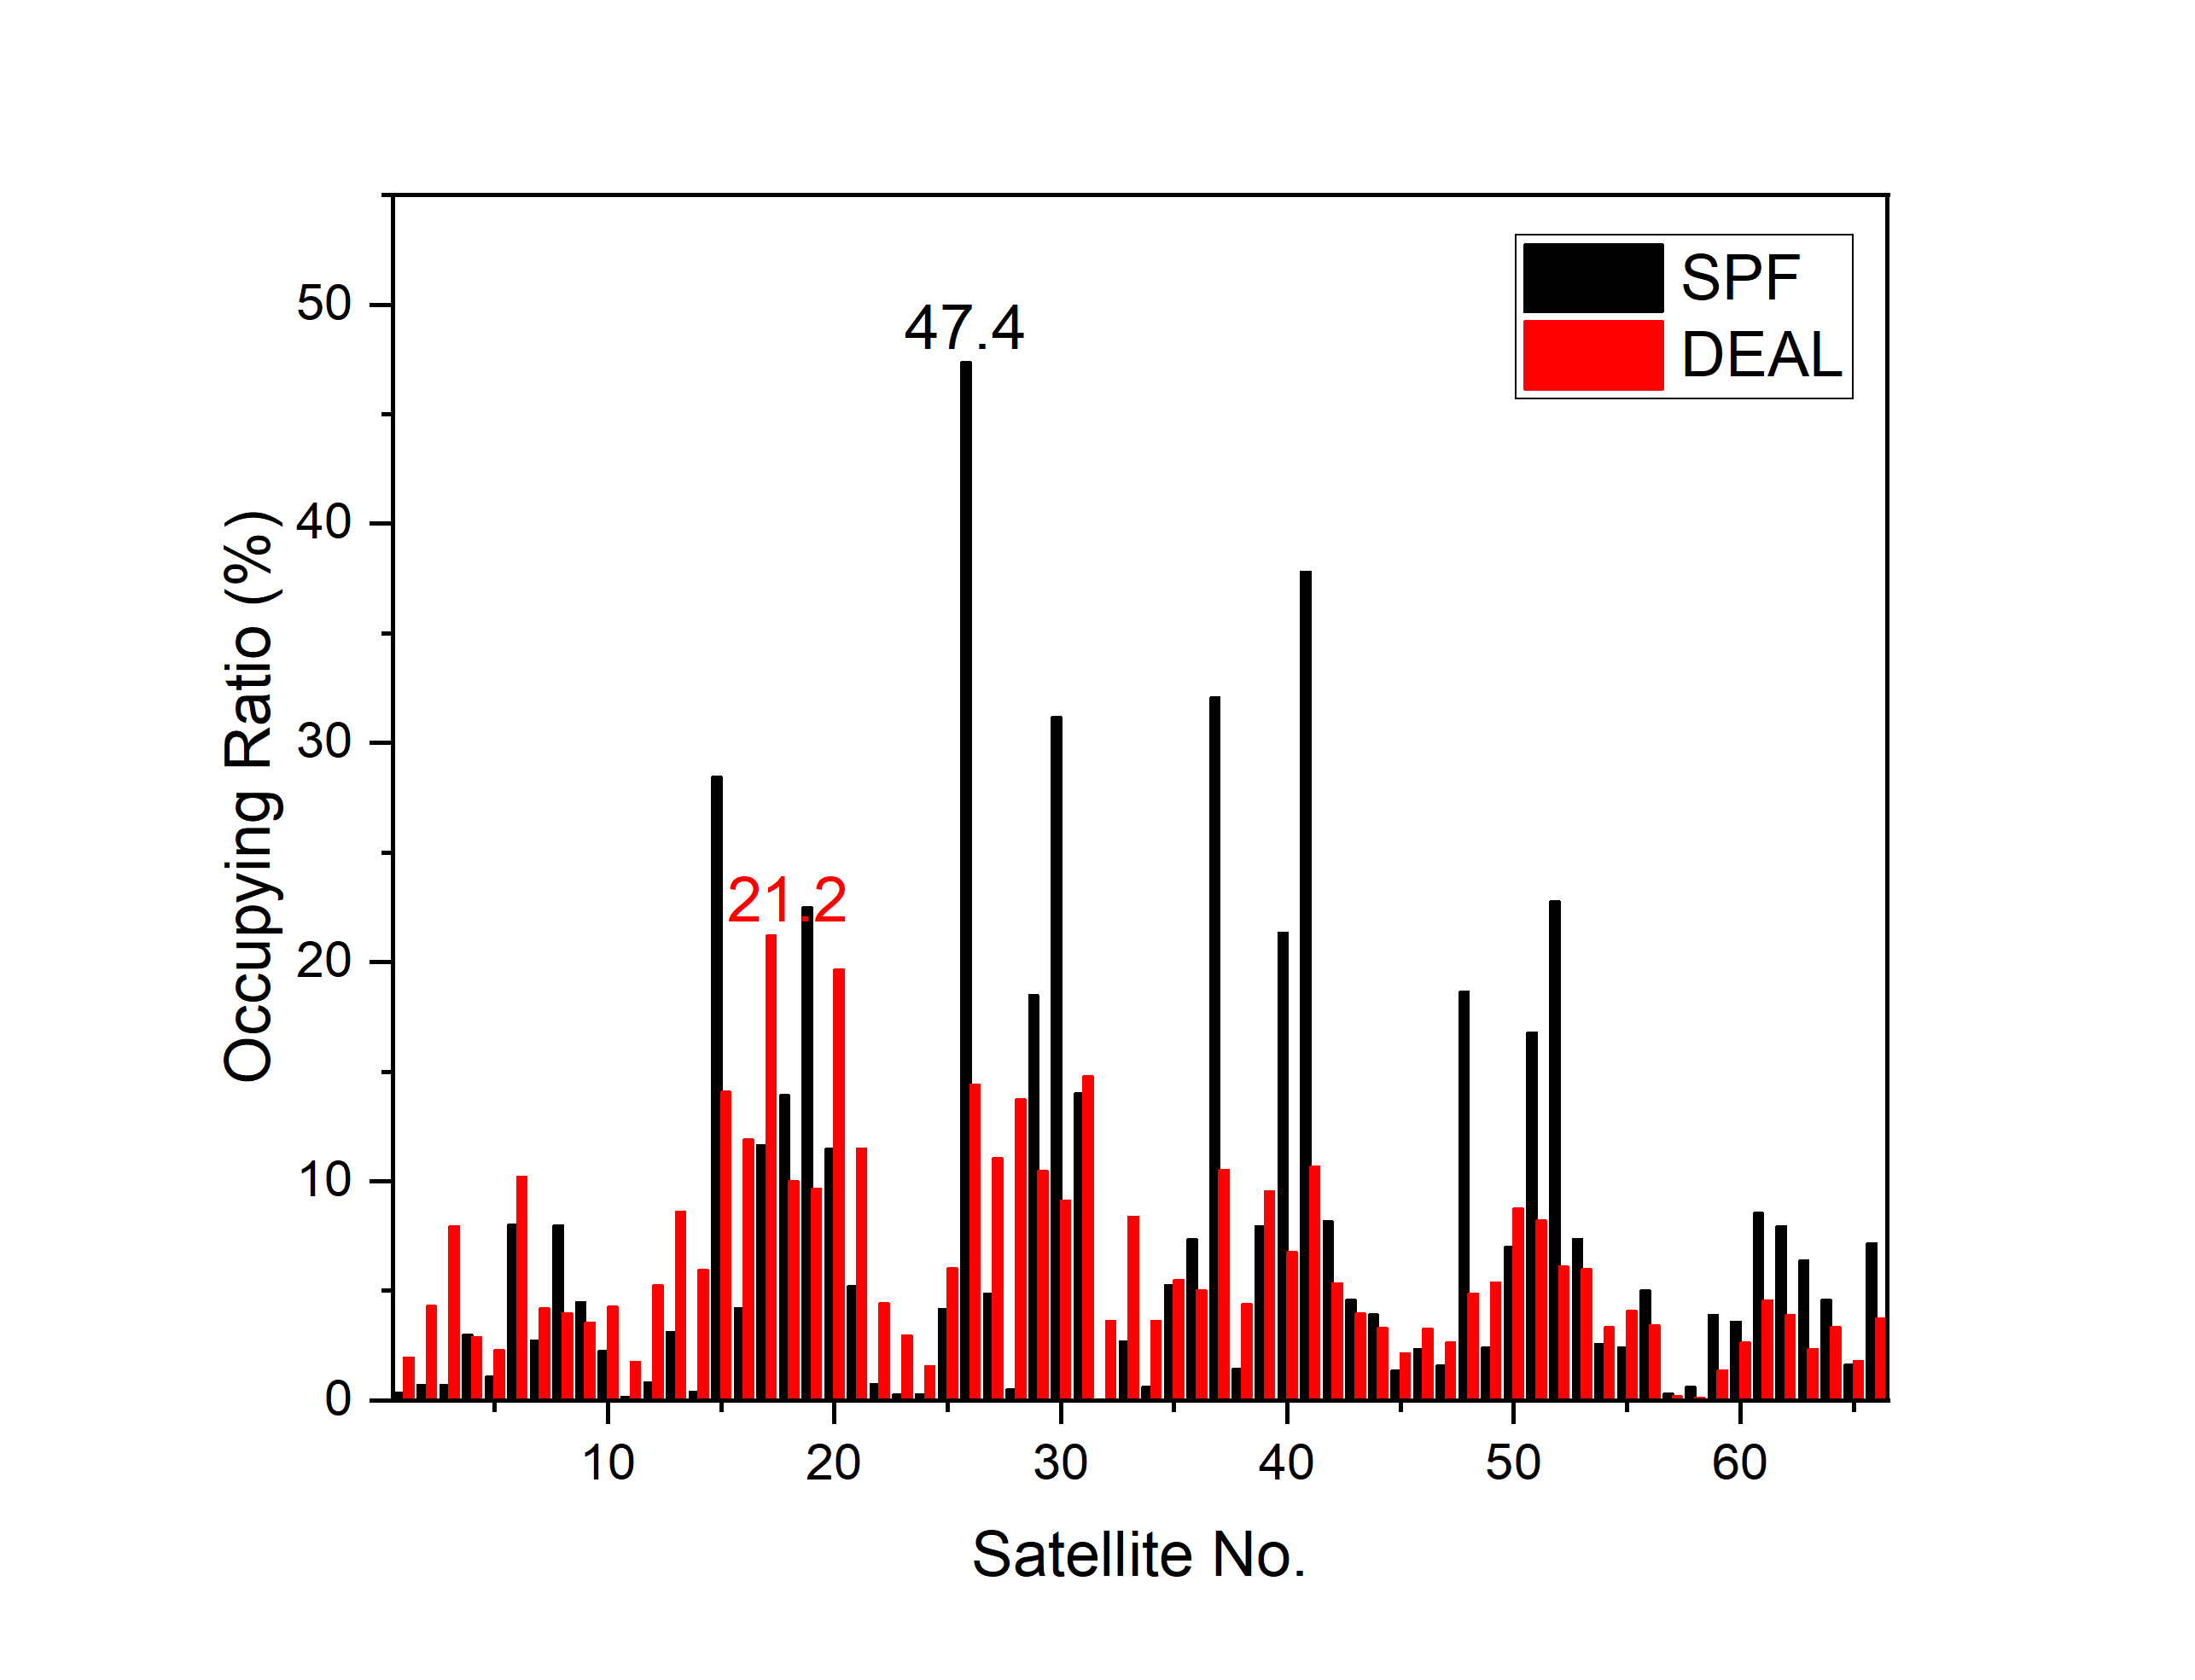
\includegraphics[width=.8\linewidth]{fig/simulation/queue/Occupying ratio of each satellite.png}
		\label{fig:ORES}
		}
	\subfigure[]{
		\centering
		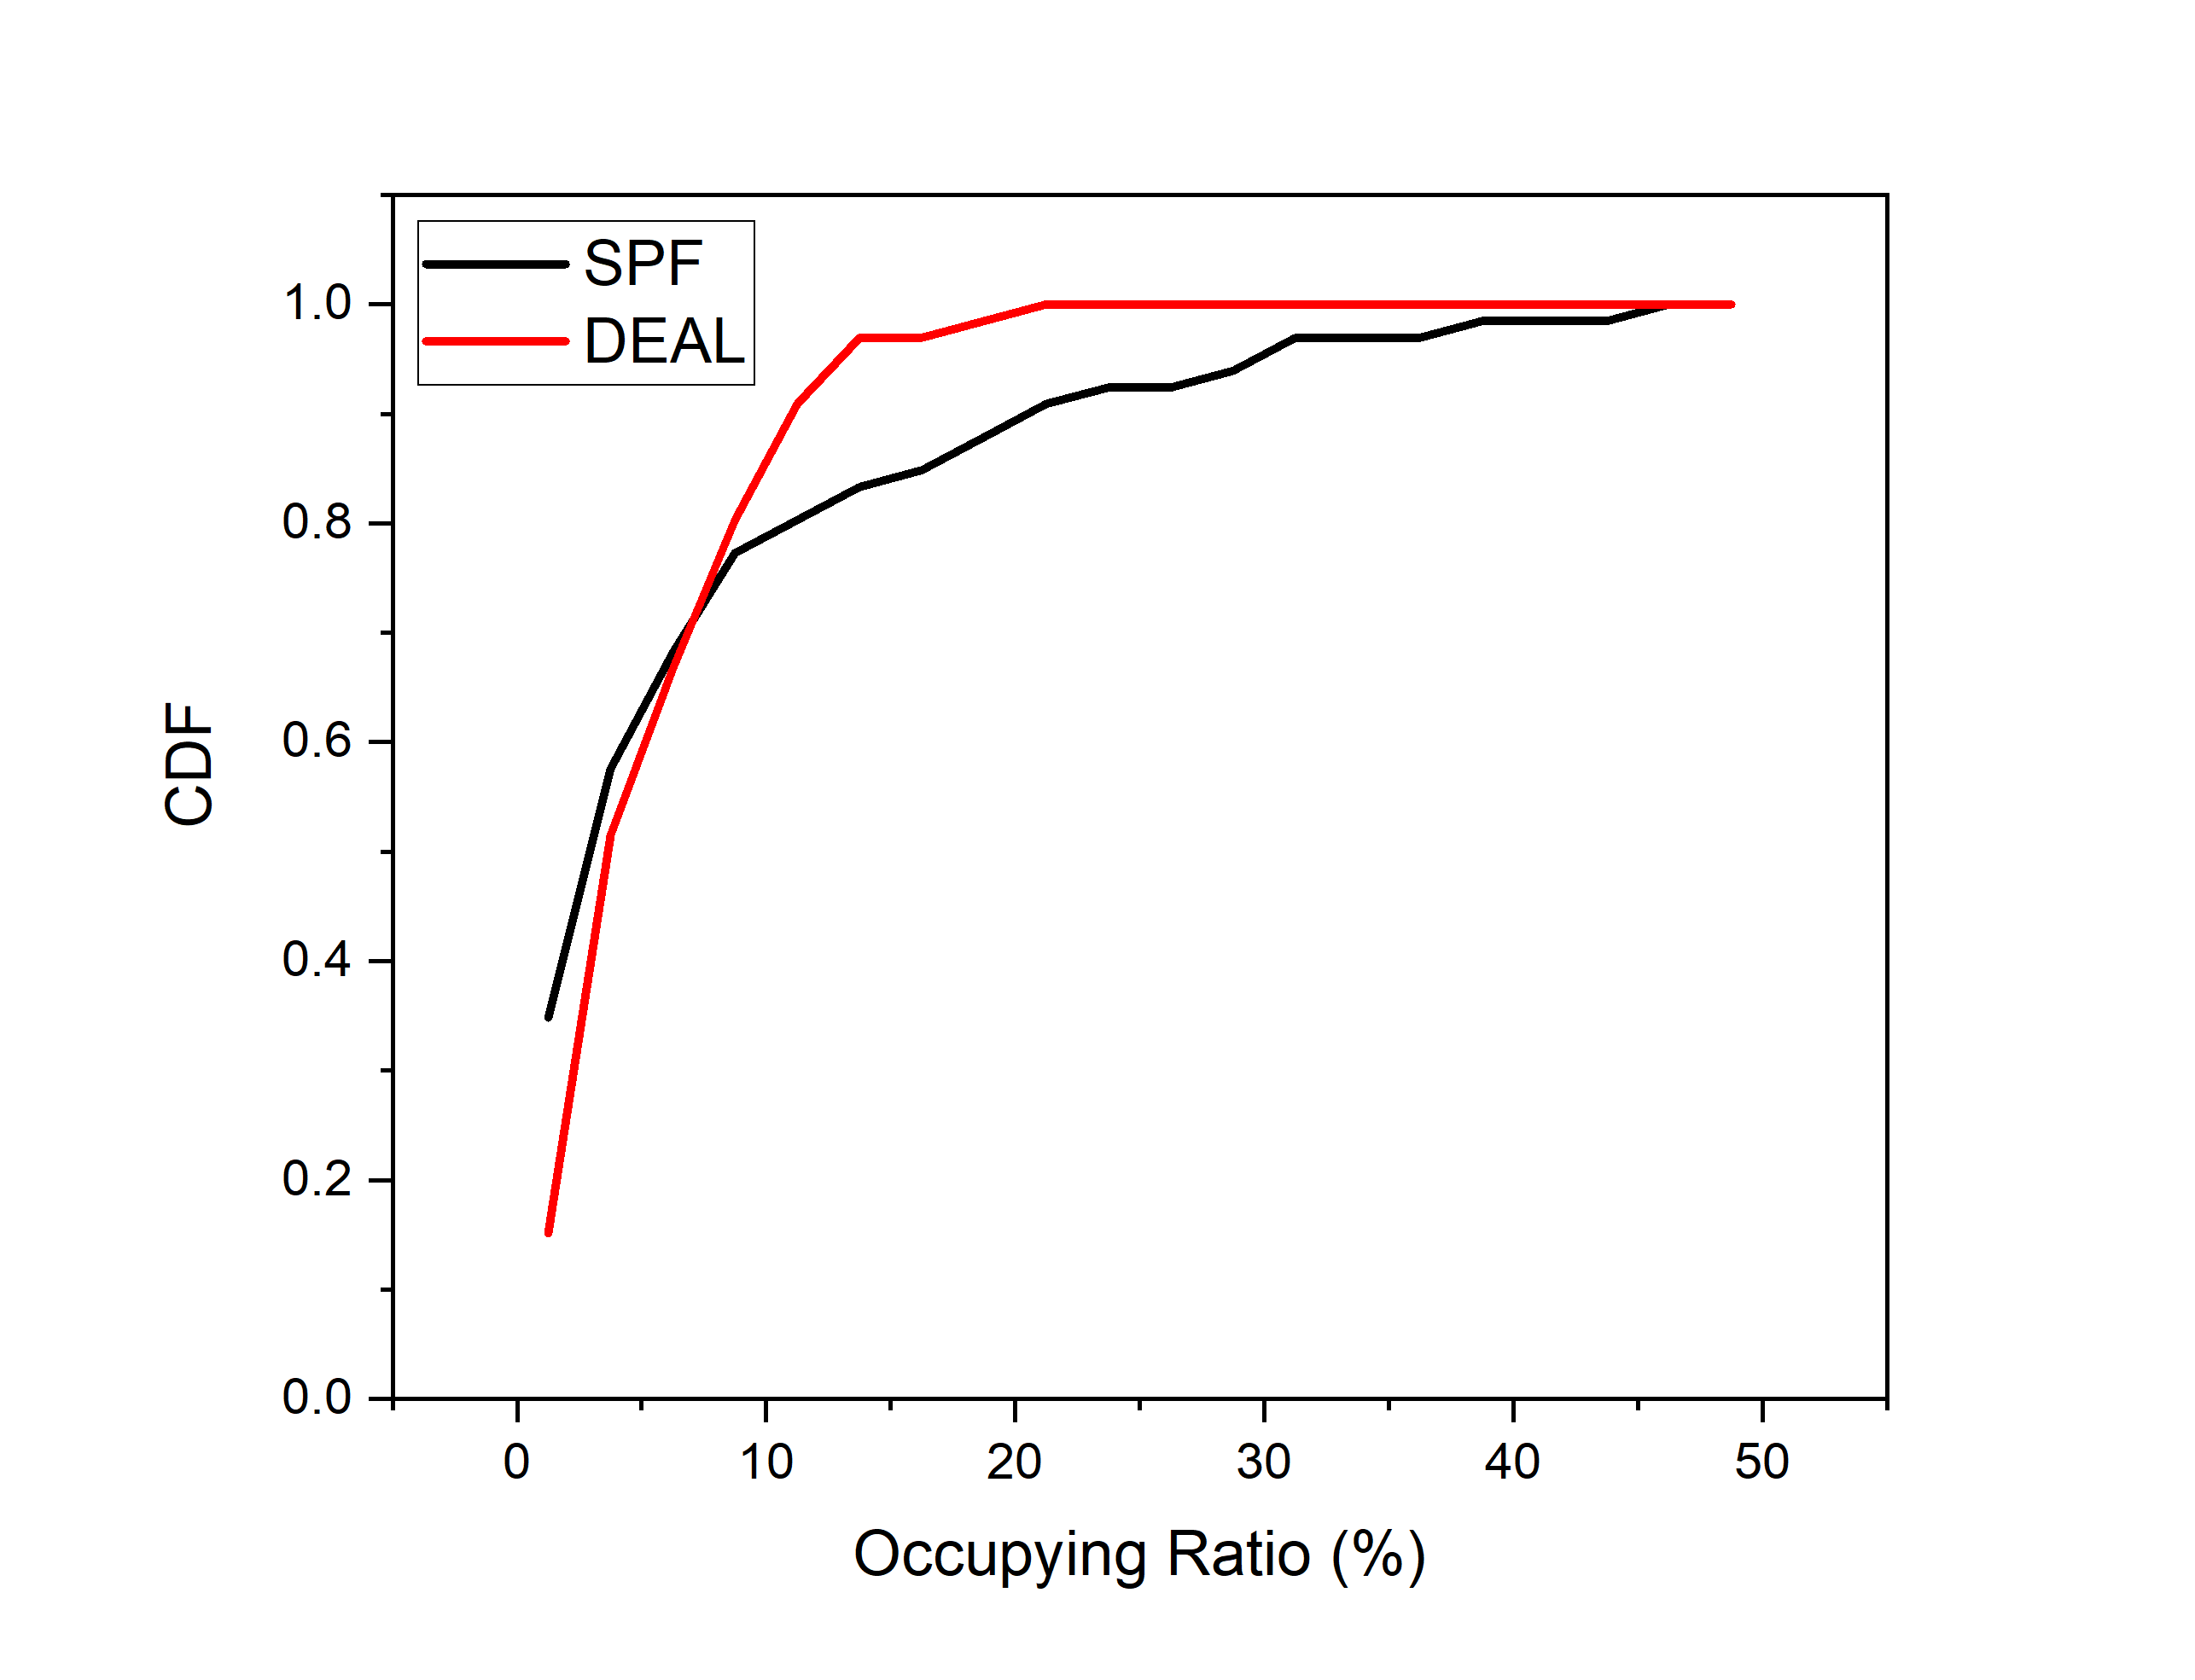
\includegraphics[width=.8\linewidth]{fig/simulation/queue/CDF of Occupying ratio.png}
		\label{fig:CDFOR}
		}
		
\caption{Occupying ratio (a) Ocuppying ratio of each satellite (b) CDF of ocuppying ratio}
\label{fig:OR}
\end{figure}

%*******************************************************************************************************************
%*      Section 7                                                                                                     
%*******************************************************************************************************************
%%%%%%%%%%%%%%Conclusion%%%%%%%%%%%%%%
\section{Conclusion}

In this paper, we proposed a Distributed Energy-Aware Load Balancing Routing Algorithm for LEO satellite network. Considering the energy is essential in the satellite networks. According to DEAL, the charging and discharging rate in LEO satellite batteries decrease, as it translates directly into cost savings. Furthermore, DEAL considers not only energy but also congestion level and ISL instability. The performance has been evaluated considering packet delivery ratio, occupying ratio of buffer queues, end-to-end delay, link utilization, and the remaining energy of satellites. Compared with the SPF algorithm, DEAL can achieve a better packet delivery ratio, load balancing, and system lifetime.

%---------- Input your reference here ---------
\bibliographystyle{IEEEtran}
\bibliography{Bibliography}

%%%%%%%%%%%%%%%%%%%%%%%%%%%%%%%%%%%%%%%%%%%%%%%%
%%%%%%%%%%%%%%%%%%%%%%%%%%%%%%%%%%%%%%%%%%%%%%%%
%----------- Input your appendix here  -----------
%%%%%%%%%%%%%%Appendix%%%%%%%%%%%%%%
%\input{Appendix}

%----------- Input your Figure chapter here  -----------
%\input{EndFigTab} 
%chapter cite  == \include
%\include{EndFigTab}
{
\begin{IEEEbiography}[{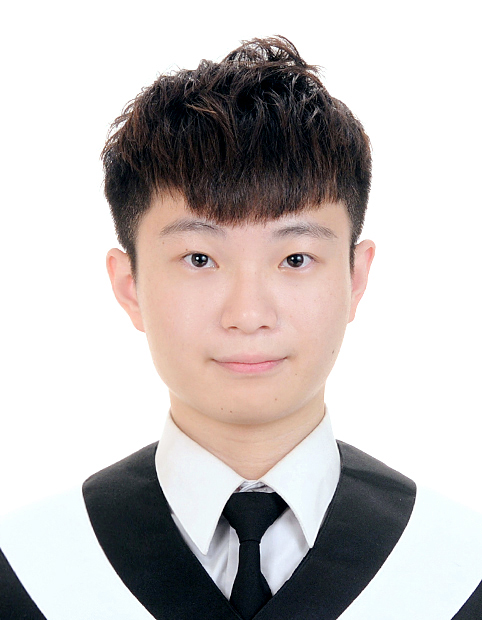
\includegraphics[width=1in,height=1.25in,clip,keepaspectratio]{pic/HCY.jpg}}]
{Chi-Yuan Huang}
received the M.S. degree in the Department of Computer Science and Information Engineering form National Central University, Taiwan, in 2021. His research interests include satellite network systems and wireless networks.
\end{IEEEbiography}

\vspace{-35pt}

\begin{IEEEbiography}[{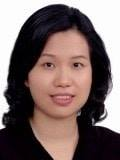
\includegraphics[width=1in,height=1.25in,clip,keepaspectratio]{pic/GYC.jpg}}]{Guey-Yun Chang}
received the B.S. and M.S. degrees in Computer Science and Information Engineering from National Taiwan Normal University, Taiwan, in 1995 and 1998, respectively, and the Ph.D. degree in Computer Science and Information Engineering from National Taiwan University, Taiwan, in 2005. Currently, she is a  professor at the Department of Computer Science and Information Engineering, National Central University, Taiwan. Her research interests include cognitive radio networks and wireless sensor networks.
\end{IEEEbiography}


\end{document}
